%==================================================================
% EAAI submission — Causal Frequency-Band Identification and OOD
% Evaluation for Vibration-Based Water Leak Detection
% Class file: elsarticle.cls (Elsevier, 2024)
%==================================================================
% EAAI requires single-column format (desk-rejection criterion).
% `3p` = single-column preprint layout in elsarticle.cls.
\documentclass[3p,times,authoryear]{elsarticle}

\usepackage{amsmath,amssymb,amsthm}
\usepackage{graphicx}
\usepackage{booktabs}
\usepackage{multirow}
\usepackage{xcolor}
\usepackage{adjustbox}
\usepackage{tikz}
\usetikzlibrary{arrows.meta,calc,positioning,fit,backgrounds}
\usepackage{subcaption}
\usepackage{placeins}
\usepackage{url}
\usepackage{hyperref}
\hypersetup{colorlinks=true, linkcolor=blue!50!black,
            citecolor=blue!50!black, urlcolor=blue!50!black}

\graphicspath{{../results/figs/}{./figures/}}

\newtheorem{definition}{Definition}
\newtheorem{proposition}{Proposition}
\theoremstyle{remark}
\newtheorem{remark}{Remark}

\journal{Engineering Applications of Artificial Intelligence}

\begin{document}
\begin{frontmatter}

\title{Shortcut Audit, Causal Bands, and an Out-of-Distribution
Recipe for Vibration-Based Water Leak Detection}

\author[1]{Suan Lee\corref{cor1}}
\ead{suanlee@semyung.ac.kr}
\cortext[cor1]{Corresponding author. Tel.: +82-43-649-1273.}

\affiliation[1]{organization={School of Computer Science,
                              Semyung University},
                addressline={65 Semyung-ro},
                city={Jecheon},
                postcode={27136},
                country={Republic of Korea}}

\begin{abstract}
A 99\,\% accuracy reported on the Korean AI~Hub water-pipe leak
benchmark collapses to weighted accuracy 56.8\,\% and macro-F1
0.304 under realistic deployment shift~---~and a four-rule lookup
that ignores the entire vibration spectrum already reaches
99.77\,\%. Tabular machine-learning pipelines for water-pipe leak
detection on vibration data routinely report such row-level
accuracies, yet they rarely survive field deployment.
The AI contribution of this paper is a reusable methodology for
auditing identifier shortcuts and quantifying out-of-distribution
(OOD) brittleness in any sensor-ML benchmark; the engineering
contribution is a deployment-candidate leak-typing recipe for municipal
water-utility networks. The methodology is instantiated on the
Korean AI~Hub vibration benchmark (70{,}384 recordings, 49 sites,
12 administrative regions) used in the author's prior study
(Lee \&~Kim 2023). Four findings. (i)~A four-probe shortcut audit: a rule-based
identifier lookup that ignores the entire vibration spectrum
reproduces 99.77\,\% validation accuracy, within 0.02 percentage
points of the published state of the art. (ii)~A three-tier OOD
ladder (row-CV $\rightarrow$ GroupKFold-by-site
$\rightarrow$ Leave-One-Region-Out) plus a 16-fold county-level
ablation: under Leave-One-Region-Out, XGBoost falls from 94.0\,\%
to weighted 56.8\,\% accuracy and macro-F1~0.304. (iii)~Three
independent attribution methods converge on \textbf{121--422~Hz}
as the robustly generalisable leak band (termed ``causal'' in the
operational OOD sense throughout this paper), with 422--1470~Hz
exposed as an active confounder whose removal \emph{improves}
OOD macro-F1; the finding is validated against seven additional
baselines, including
gradient-boosted ensembles, attentive tabular deep learning, and
domain-alignment methods (correlation alignment, domain-adversarial
training, and maximum-mean-discrepancy generalisation).
(iv)~A multi-seed deployment recipe: a tree-only soft average of
flat and hierarchical XGBoost on 57 causal features attains OOD
macro-F1 \textbf{0.4326} with perfect normal-class recall; the
strongest deep alternative (an MLP trained with group
distributionally robust optimisation, GroupDRO) reaches only
$0.358 \pm
0.013$ across five seeds. The audit protocol is independently
re-applied to nine external public sensor benchmarks
(UCI~SECOM~\cite{mccann2008secom},
UCI~HAR~\cite{anguita2013har}, and the seven machines of
MIMII-DG~\cite{dohi2022mimii}) and shown to discriminate
shortcut-laden from clean
benchmarks rather than blanket-flagging vibration data. The
full audit protocol, multi-seed harness, and deployment recipe
are released for reproducibility.
\end{abstract}

\begin{keyword}
water leak detection \sep vibration sensor \sep
out-of-distribution evaluation \sep shortcut learning \sep
causal feature selection \sep smart-water-grid
\end{keyword}

\end{frontmatter}

%==================================================================
\section{Introduction}\label{sec:intro}

Non-revenue water loss from leaking metal and non-metal
distribution pipes is a persistent infrastructure problem with
substantial economic and environmental cost worldwide, particularly
acute in aging urban networks. Acoustic leak detection using
low-cost vibration sensors mounted at water meters, valves, and
hydrants has emerged as one of the most widely deployed monitoring
strategies because of its low installation cost,
non-invasiveness, and compatibility with cellular
telemetry~\cite{hunaidi2000plastic,ismail2019review}.
On the sensing side, the dominant trend over the past decade has
been to replace hand-tuned threshold rules with tabular machine
learning (ML) applied to frequency-domain features of the
vibration spectrum~\cite{shukla2020leakage,fereidooni2021hybrid,
cody2020leak,liu2019leakage}.

The study that motivates the present follow-up is the author's
own previous work on the Korean AI~Hub water-pipeline
benchmark~\cite{lee2023leak}, in which eight tabular models were
compared across four feature regimes and an XGBoost classifier
reached 99.79\,\% accuracy under stratified 10-fold
cross-validation. The goal of that paper was a comparative
benchmark of off-the-shelf models on newly curated sensor data,
and within its stated evaluation protocol the result is faithful.
However, on subsequently attempting to operationalise the same
pipeline for field use by a municipal water utility, two
practical obstacles became visible. First, the 10-fold row-level
split placed multiple recordings from the same physical sensor in
both train and test folds, so the reported accuracy actually
measured within-sensor repeatability more than cross-sensor
generalisation. Second, as the shortcut-learning literature in
medical imaging~\cite{zech2018pneumonia,degrave2021covid,
geirhos2020shortcut,damour2022underspec} and natural-image
recognition~\cite{beery2018terra} has documented, sensor-ML
models routinely latch onto identifier-like features that
correlate perfectly with the label in the training distribution
but do not represent any physical signal.

\paragraph{Scope of this paper.}
This paper addresses that gap with a reusable AI methodology
and a deployment-candidate recipe. Treating the AI~Hub benchmark as
one carefully studied case rather than the exclusive object of
study, four contributions of broader interest to engineering AI
practitioners are made.

\begin{enumerate}
\item \textbf{A reusable four-probe shortcut-audit protocol for
sensor-ML benchmarks.} Per-sensor label purity, class-lookup
reconstruction, sensor train/test overlap, and a
meta-column-override probe. On AI~Hub, a four-rule identifier
lookup that ignores the entire vibration spectrum reproduces
99.77\,\% validation accuracy --- within 0.02 percentage points
of the published state of the art~\cite{lee2023leak}.

\item \textbf{A three-tier out-of-distribution evaluation
protocol with a county-level extension.} Row-CV
$\rightarrow$ GroupKFold-by-site $\rightarrow$
Leave-One-Region-Out (LORO) over 12 \textit{gwangyeoksi-do}, plus a 16-fold
Leave-One-County-Out over the eligible \textit{sigungu} (16 of 36 with
$\geq 4$ leak classes present). Under LORO
the XGBoost classifier of~\cite{lee2023leak} falls to weighted
accuracy 56.8\,\% and macro-F1 0.304.

\item \textbf{Identification of the robustly generalisable spectral
signature of leak noise.} Three independent attribution
methods --- bootstrap permutation importance,
TreeSHAP~\cite{lundberg2017shap}, and multi-region
replication --- converge on the \textbf{121--422~Hz} band,
broadly consistent with published plastic-pipe
acoustics~\cite{hunaidi2000plastic,almeida2014leak,
gao2017model}. The 422--1470~Hz range is exposed as an active
confounder whose permutation \emph{improves} OOD macro-F1.
Following~\cite{arjovsky2019irm,scholkopf2021causal}, the
selected band is called ``causal'' in the operational sense of
``necessary for OOD generalisation'' throughout this paper
(Remark~\ref{rem:causal}).

\item \textbf{A multi-seed deployment recipe with a full
computational-cost analysis.} Restricting the input to 57
causal features and combining a flat causal XGBoost with a
hierarchical (binary energy gate $+$ 4-class causal typer) via
a pre-specified soft average attains OOD macro-F1
\textbf{0.4326} with perfect normal-class recall on the canonical
LORO fold. The recipe is compared on macro-F1 against seven
additional baselines (LightGBM~\cite{ke2017lightgbm},
CatBoost~\cite{prokhorenkova2018catboost},
TabNet~\cite{arik2021tabnet}, Random~Forest~\cite{breiman2001rf},
DeepCORAL~\cite{sun2016coral}, DANN~\cite{ganin2016dann},
MMD-DG~\cite{li2018mmddg}); training time, inference latency per
1{,}000 rows, peak RAM and peak GPU memory are reported for the
deployment-relevant subset (XGBoost flat, XGBoost hierarchical,
tree-ensemble, LightGBM, CatBoost, Random~Forest, and the
multi-layer perceptron (MLP) / one-dimensional convolutional
neural network (1D-CNN) backbones under empirical risk
minimisation (ERM)).
\end{enumerate}

\begin{figure*}[!htbp]
\centering
\resizebox{0.95\textwidth}{!}{% fig_overview.tex -- Figure 1 (Overview), native TikZ.
% Compact layout: short stage cards, tight spacing to context strip.

\definecolor{ctxfill}{HTML}{FFF8DC}
\definecolor{delvfill}{HTML}{ECF0F1}
\definecolor{s1fill}{HTML}{E8F0FE}\definecolor{s1txt}{HTML}{C0392B}
\definecolor{s2fill}{HTML}{FDECEA}\definecolor{s2txt}{HTML}{C0392B}
\definecolor{s3fill}{HTML}{E9F7EF}\definecolor{s3txt}{HTML}{1E8449}
\definecolor{s4fill}{HTML}{EFE6F7}\definecolor{s4txt}{HTML}{1A5FB4}
\definecolor{darkborder}{HTML}{2C3E50}

\begin{tikzpicture}[
    font=\footnotesize,
    box/.style={rounded corners=4pt, draw=darkborder!85, line width=0.7pt},
    stage/.style={rounded corners=5pt, draw=darkborder!85, line width=0.8pt,
                  minimum width=4.45cm, minimum height=4.2cm, anchor=north west},
    headband/.style={rounded corners=3pt, fill=white,
                     align=center, font=\bfseries\normalsize,
                     minimum width=4.0cm, minimum height=0.8cm, anchor=south},
    arr/.style={-{Stealth[length=2.5mm,width=2mm]}, line width=1pt, draw=darkborder!85},
    downarr/.style={-{Stealth[length=3mm,width=2.5mm]}, line width=1.3pt,
                    draw=darkborder!85},
]

% ========== Context strip ==========
\node[box, fill=ctxfill, inner sep=8pt, anchor=north west,
      text width=18.6cm, align=left] (ctx) at (0,0) {%
  \textbf{\normalsize Input and motivating question}\par\vspace{3pt}
  \textbullet~Korean AI\,Hub water-pipe vibration benchmark:
    70{,}384 recordings, 49 sites, 12 administrative regions,
    5 leak classes.\par
  \textbullet~Prior reported ceiling (row-level 10-fold CV,
    Lee \& Kim 2023): XGBoost accuracy 0.9979.\par
  \textbullet~Practitioner's question: does that number hold on a
    new sensor, at an unseen site, or in a different region?
};

% ========== Four stage cards (half-height, directly below context) ==========
\def\ys{-2.25}

\node[stage, fill=s1fill] (s1box) at (0.00, \ys) {};
\node[anchor=north west, text width=4.1cm, inner sep=6pt]
     at (s1box.north west) {%
  {\LARGE\bfseries 1}\hspace{4pt}{\bfseries\normalsize Shortcut audit}\par
  \vspace{5pt}
  \textbullet~2{,}671 sensors each map to one class\par
  \textbullet~97.96\% val sid in train
};
\node[headband, text=s1txt]
     at ($(s1box.south)+(0, 0.15)$) {Zero-ML = 99.77\% val};

\node[stage, fill=s2fill] (s2box) at (4.82, \ys) {};
\node[anchor=north west, text width=4.1cm, inner sep=6pt]
     at (s2box.north west) {%
  {\LARGE\bfseries 2}\hspace{4pt}{\bfseries\normalsize Three-tier OOD}\par
  \vspace{5pt}
  \textbullet~Row 0.94 \;$\to$\; Site 0.55 \;$\to$\; LORO 0.57\par
  \textbullet~Chungbuk (5 cls): macro-F1 0.4148
};
\node[headband, text=s2txt]
     at ($(s2box.south)+(0, 0.15)$) {$-$39~pp drop};

\node[stage, fill=s3fill] (s3box) at (9.64, \ys) {};
\node[anchor=north west, text width=4.1cm, inner sep=6pt]
     at (s3box.north west) {%
  {\LARGE\bfseries 3}\hspace{4pt}{\bfseries\normalsize Causal spectral}\par
  \vspace{5pt}
  \textbullet~121--422~Hz = real leak signal\par
  \textbullet~422--1470~Hz = active confounder\par
  \textbullet~Confirmed 3$\times$ (perm, SHAP, 4-fold)
};
\node[headband, text=s3txt]
     at ($(s3box.south)+(0, 0.15)$) {121--422~Hz (SHAP 40\%)};

\node[stage, fill=s4fill] (s4box) at (14.46, \ys) {};
\node[anchor=north west, text width=4.1cm, inner sep=6pt]
     at (s4box.north west) {%
  {\LARGE\bfseries 4}\hspace{4pt}{\bfseries\normalsize Deployment recipe}\par
  \vspace{5pt}
  \textbullet~Stage~1 normal gate: 100\% OOD recall\par
  \textbullet~Stage~2 causal 4-class typer\par
  \textbullet~Soft-averaged tree ensemble
};
\node[headband, text=s4txt]
     at ($(s4box.south)+(0, 0.15)$) {Best macro-F1 = 0.4326};

% Arrows between stages
\draw[arr] (s1box.east) -- (s2box.west);
\draw[arr] (s2box.east) -- (s3box.west);
\draw[arr] (s3box.east) -- (s4box.west);

% ========== Deliverable strip ==========
\def\yd{-6.85}
\node[box, fill=delvfill, inner sep=7pt, anchor=north west,
      text width=18.7cm, align=left] (delv) at (0, \yd) {%
  \textbf{\small Deliverables for practitioners}\par\vspace{2pt}
  \small
  $\blacktriangleright$~Open-source pipeline (MIT): 22 scripts,
    13 raw-metric JSONs, figures, LaTeX source.\par
  $\blacktriangleright$~Reusable shortcut-audit protocol.\par
  $\blacktriangleright$~Hierarchical + ensemble recipe with perfect
    OOD normal-class recall.
};

\end{tikzpicture}
}
\caption{\textbf{Overview of the study.} The paper proceeds as a
four-stage pipeline from the benchmark ceiling reported
in~\cite{lee2023leak} to a deployment-candidate recipe.
(1)~A zero-ML identifier lookup reproduces the reported 99.77\,\%
accuracy, so the signal contribution to the headline number is
negligible.
(2)~A three-tier OOD evaluation exposes a $\sim$39-percentage-point
accuracy drop between row-level and GroupSite-by-site
cross-validation, and a further drop to weighted accuracy
56.8\,\% under Leave-One-Region-Out.
(3)~Three independent attribution methods (permutation importance,
TreeSHAP, cross-region bootstrap) converge on \textbf{121--422~Hz}
as the generalisable leak-signal band, with 422--1470~Hz identified
as an active confounder.
(4)~A pre-specified soft-probability average of flat and
hierarchical XGBoost on the 57 causal features attains OOD
macro-F1 \textbf{0.4326} with perfect normal-class recall on the
canonical Chungbuk fold.\label{fig:overview}}
\end{figure*}

Figure~\ref{fig:overview} summarises the four stages of the
study as a single pipeline diagram, anchoring each stage to
the headline quantitative result that section will defend.

The remainder of the paper is organised as follows.
Section~\ref{sec:related} surveys the four bodies of literature
this work intersects (vibration leak detection, shortcut learning,
OOD generalisation, tabular deep learning). Section~\ref{sec:methodology}
formalises the methodology with four definitions and an
applicability checklist. Section~\ref{sec:setup} describes the
dataset, multi-seed protocol, hardware, and reproducibility
infrastructure. Section~\ref{sec:results} presents the
experimental results organised around seven research questions.
Section~\ref{sec:engineering} discusses engineering implications
and translates the recipe into operational metrics, a
cost-benefit estimate, and a SCADA/IoT integration template.
Section~\ref{sec:threats} catalogues threats to validity and
failure modes. Section~\ref{sec:conclusions} concludes.

%==================================================================
\section{Related Work}\label{sec:related}

\subsection{Vibration-Based Leak Detection}

Acoustic signatures of water leaks in buried pipes have been
studied since at least the late 1990s. For plastic pipes,
\citet{hunaidi2000plastic} reported that leak-noise energy is
concentrated below roughly 600~Hz, with the precise band
depending on pipe material, diameter, and internal pressure.
\citet{almeida2014leak} quantified the acoustic filtering
introduced by sensor mounting and pipe-wall damping in buried
plastic pipes; \citet{gao2017model} improved the shape of the
cross-correlation function for time-delay-based leak detection
in plastic distribution pipes by removing pipe-resonance
effects, broadening the usable bandwidth of the analysis.
\citet{ismail2019review} systematically reviewed
accelerometer-based approaches, classifying the literature into
threshold methods, signal-processing methods (cross-correlation,
EMD, wavelet), and machine-learning methods.

Recent representative ML works include
\citet{shukla2020leakage} (supervised classification of
acceleration signals), \citet{fereidooni2021hybrid}
(hybrid model-based methods for large distribution networks),
\citet{cody2020leak} (deep autoencoders on hydroacoustic
spectrograms), \citet{liu2019leakage} (machine-learning over
wireless-sensor-network signals), and \citet{tariq2022leak}
(data-driven leak detection with MEMS-based accelerometers).
Korean studies on the AI~Hub
benchmark~\cite{lee2023leak} have reported above-99\,\%
accuracy with tree ensembles such as
XGBoost~\cite{chen2016xgboost} and Random
Forest~\cite{breiman2001rf}. The reported numbers are measured
under stratified row-level cross-validation on a merged-and-
resplit training set; no published evaluation on the benchmark
has used a sensor-group, site-group, or region-group holdout,
and none has audited for identifier shortcuts. This paper
supplies that evaluation.

\subsection{Shortcut Learning and Spurious Correlation}

The shortcut-learning framework~\cite{geirhos2020shortcut}
provides a vocabulary for the failure mode in which a supervised
model latches onto superficial features that correlate with the
label in training but do not represent the underlying task.
\citet{zech2018pneumonia} showed that a deep pneumonia
classifier was effectively detecting the hospital of origin via
metadata artefacts in radiographs;
\citet{degrave2021covid} documented analogous shortcut behaviour
in COVID-19 chest-X-ray classifiers; \citet{beery2018terra}
demonstrated that animal-species recognisers trained on wildlife
camera imagery rely heavily on background context.
\citet{damour2022underspec} frame the phenomenon more generally:
many equally accurate models on the training distribution can
behave very differently under deployment shift.
\citet{liu2021jtt} propose Just-Train-Twice as a
group-information-free worst-group remedy. Formal shortcut
audits have been rare in the sensor-ML literature; this paper
adapts the protocol to a vibration-based leak-detection
benchmark and finds a particularly extreme form of the
pathology.

\subsection{Out-of-Distribution Generalisation and Domain Alignment}

Loss-level invariance regularisers are the canonical algorithmic
response to spurious correlations.
IRM~\cite{arjovsky2019irm} adds a penalty that discourages
representations whose risk varies across training environments;
GroupDRO~\cite{sagawa2020groupdro} minimises the worst-case
per-environment loss; REx~\cite{krueger2021rex} penalises the
variance of per-environment risks; Fishr~\cite{rame2022fishr}
operates on gradient variances. The empirical reliability of
these methods has been repeatedly
questioned~\cite{gulrajani2021dg,rosenfeld2021irm}: with few
or uneven environments they often fail to beat plain Empirical
Risk Minimisation on OOD test sets.

A complementary line of work --- domain-adaptation and
domain-generalisation methods --- aligns feature distributions
between source and target environments. DeepCORAL minimises the
Frobenius distance between source and target covariance
matrices~\cite{sun2016coral}; DANN trains a domain classifier
through a gradient-reversal layer~\cite{ganin2016dann};
MMD-DG~\cite{long2015dan,li2018mmddg,gretton2012mmd} minimises the maximum mean
discrepancy across environments. Section~\ref{sec:results}
contributes evaluations of all three on the AI~Hub LORO fold.

\subsection{Tabular Deep Learning}

Tabular deep learning has matured rapidly with the introduction
of TabNet~\cite{arik2021tabnet}, NODE~\cite{popov2020node}, and
FT-Transformer~\cite{gorishniy2021ftt}. The recent survey of
\citet{borisov2024tabsurvey} reports that, on most benchmarks,
gradient-boosted decision trees (XGBoost~\cite{chen2016xgboost},
LightGBM~\cite{ke2017lightgbm},
CatBoost~\cite{prokhorenkova2018catboost}) remain competitive
with --- and frequently exceed --- the strongest deep tabular
architectures, particularly on small to medium datasets. All
three boosting variants and TabNet are included as additional
baselines on the AI~Hub fold.

\subsection{Reproducibility and Industrial AI}

Concern about empirical robustness in ML benchmarking has driven
the development of reproducibility surveys (Pineau et
al.~\cite{pineau2021reproducibility};
Henderson~\cite{henderson2018reproducibility}) and the WILDS
distribution-shift benchmark~\cite{koh2021wilds}. AI risk
frameworks for high-stakes infrastructure --- the NIST AI
RMF~\cite{nist2023airmf} and the EU AI~Act~\cite{eu2024aiact}
high-risk categorisation of critical infrastructure ---
make explicit deployment-evaluation requirements that the
shortcut-audit protocol of this paper directly supports.

%==================================================================
\section{Problem Formulation and Methodology}\label{sec:methodology}

\subsection{Problem Setting and Notation}

Let $\mathcal{D} = \{(x_i, y_i, s_i, e_i)\}_{i=1}^{N}$ denote a
sensor-ML benchmark, where $x_i \in \mathbb{R}^{d}$ is the
feature vector, $y_i \in \{1,\dots,C\}$ is the class label,
$s_i$ is a per-sensor identifier, and
$e_i \in \{1,\dots,E\}$ is a higher-order group identifier
(site, region). Let $\ell$ denote a class-weighted softmax
cross-entropy with inverse-frequency class weights
$w_c = N / (CN_c)$, $R(\theta) = N^{-1}\sum_i \ell(f_\theta(x_i),
y_i)$ the pooled risk, and
$R_e(\theta) = N_e^{-1}\sum_{i:e_i=e} \ell(f_\theta(x_i), y_i)$
the per-environment risk. The feature vector is assumed to partition
into $G$ disjoint physical groups
$x = (x^{(1)}, \dots, x^{(G)})$ (e.g.\ frequency bands,
multivariate channels, segments of a trajectory).

\subsection{Definition 1: Identifier-Shortcut Sensor Benchmark}

\begin{definition}[Identifier-shortcut benchmark]\label{def:shortcut}
A sensor-ML benchmark $\mathcal{D}$ together with a row-level
train/validation split admits an \emph{identifier shortcut} of
strength $(\epsilon, \delta)$ if there exists a deterministic
mapping $h \colon (s, m) \mapsto y$, depending only on the
identifier $s$ and any meta-columns $m$ (timestamp, sample-rate
flags, etc.) but not on $x$, such that
\[
  \frac{1}{N_{\mathrm{val}}} \sum_{i \in \mathrm{val}}
  \mathbb{1}\bigl[h(s_i, m_i) = y_i\bigr] \;\geq\; 1 - \epsilon,
\]
and $\Pr\bigl[s_i \in \mathrm{train}\,|\,i \in \mathrm{val}\bigr]
\;\geq\; 1 - \delta$.
\end{definition}

A benchmark with $(\epsilon, \delta) \approx (0, 0)$ contains a
near-perfect identifier shortcut: any reported validation
accuracy is bounded above $1 - \epsilon$ by $h$ alone, so the
contribution of any model trained on $x$ is at most $\epsilon$ in
absolute accuracy. Section~\ref{sec:results} demonstrates that
the AI~Hub benchmark with the standard split satisfies
$(\epsilon, \delta) \leq (0.0023, 0.0204)$,
which means the published 99.79\,\% accuracy~\cite{lee2023leak}
is within rounding of the lookup ceiling.

\subsection{Definition 2: Four-Probe Shortcut Audit}\label{sec:method-audit}

\begin{definition}[Four-probe shortcut audit]\label{def:audit}
Given $\mathcal{D}$ and a row-level train/val split,
the \emph{four-probe shortcut audit} computes:
\begin{itemize}
\item \textbf{P1 (per-sensor label purity)}: for each training
sensor $s$, the fraction of rows at $s$ whose label matches
the modal label at $s$. Median purity $\geq 0.95$ flags
single-class sensors.

\item \textbf{P2 (class-lookup reconstruction)}: build
$\widehat{h}_{\mathrm{lookup}}(s) := \arg\max_y
\Pr_{\mathrm{train}}(y \mid s)$ and apply it to validation
rows. Report the coverage and covered-row accuracy.

\item \textbf{P3 (sensor train/test overlap)}: the fraction of
validation sensors whose identifier $s$ also appears in the
training split.

\item \textbf{P4 (lookup + meta-column override)}: combine P2
with a rule-based override on any meta-column whose value is
deterministically associated with a specific class. Report
the resulting accuracy.
\end{itemize}
A benchmark passes the audit if no probe reaches the published
benchmark accuracy; it fails if P1, P3, and P4 jointly do.
\end{definition}

\subsection{Definition 3: Three-Tier OOD Evaluation Ladder}\label{sec:method-ood}

\begin{definition}[Three-tier OOD evaluation]\label{def:ood}
Evaluation under increasing deployment realism:
\begin{itemize}
\item \textbf{Row-CV.} Stratified $k$-fold over rows. The same
sensor's measurements may appear in both folds.
\item \textbf{GroupSite-CV.} GroupKFold by \texttt{site}, so
every test sensor has been unseen at train time. Simulates
deployment to a new installation within the same region.
\item \textbf{LORO.} Leave-One-Region-Out over the
administrative regions. Simulates deployment to a new city
or province.
\end{itemize}
The gap between row-CV and LORO on the same model gives a
quantitative measure of the deployment-shift brittleness of a
pipeline.
\end{definition}

A finer-grained Leave-One-County-Out (LOCO) protocol is also
evaluated on the AI~Hub benchmark, drawing held-out test folds
from the 36 unique \textit{sigungu} (county) codes — restricted to the 16
eligible folds with at least four leak classes present —
versus the 12 environments at the \textit{gwangyeoksi-do} (metropolitan-region)
level. LOCO tests whether more environments stabilise
gradient-based invariance regularisers
(IRM~\cite{arjovsky2019irm}, GroupDRO~\cite{sagawa2020groupdro}).

\subsection{Definition 4: Grouped Permutation Importance}\label{sec:method-perm}

\begin{definition}[Grouped permutation importance]\label{def:perm}
After training $f_\theta$ on the pooled training set, the causal
contribution of a feature group $g \in \{1,\dots,G\}$ is measured
on the held-out set by
\[
\Delta_{\mathrm{F1}}(g) =
  \mathrm{F1}\bigl(y, f_\theta(x)\bigr)
  - \mathrm{F1}\bigl(y, f_\theta(\tilde{x}^{(g)})\bigr),
\]
where $\tilde{x}^{(g)}$ permutes only the columns indexed by
group $g$. Positive $\Delta_{\mathrm{F1}}(g)$ marks $g$ as
carrying generalisable signal; negative $\Delta_{\mathrm{F1}}(g)$
marks $g$ as a confounder whose removal helps. A bootstrap
confidence interval on $\Delta_{\mathrm{F1}}(g)$ is obtained by
$B$ independent permutations of $x^{(g)}$.
\end{definition}

Definition~\ref{def:perm} is further paired with a SHAP
second-source attribution~\cite{lundberg2017shap}, declaring a
group $g$ \emph{robustly generalisable} on the test fold only if
$\Delta_{\mathrm{F1}}(g) > 0$ \emph{and} the SHAP-magnitude
share of $g$ is in the top quartile. SHAP is one of several
feature-attribution methods that could be substituted at this
step; LIME~\cite{ribeiro2016lime} offers a local-surrogate
alternative, and causal Shapley
values~\cite{janzing2020shapley} provide a stronger
interpretation when the data-generating process is partly
known~\cite{lipton2018mythos,barredo2020xai}. TreeSHAP is used here because the underlying model is a
gradient-boosted tree ensemble for which exact path-based
attribution is tractable. Causal Shapley values were not
adopted because they require a known or estimated causal
graph among features, which is unavailable for the 513
frequency bins: while the bins are physically ordered, their
conditional independence structure is not known a priori and
would need to be estimated from data --- introducing a
circularity that the simpler permutation-plus-SHAP protocol
avoids.

\begin{remark}[Use of the term ``causal'']\label{rem:causal}
Throughout this paper, a feature group is called \emph{causal}
in the operational sense that (i)~its permutation degrades OOD
macro-F1 on held-out regions, (ii)~two independent attribution
methods (permutation importance and TreeSHAP) converge on the
same group, and (iii)~the identified band (121--422~Hz) is
physically consistent with published plastic-pipe leak
acoustics~\cite{hunaidi2000plastic,almeida2014leak,gao2017model}.
This usage follows the ``necessary for OOD generalisation''
convention common in the distribution-shift
literature~\cite{arjovsky2019irm,scholkopf2021causal} and does
\emph{not} imply a formal interventionist causal claim in the
structural-causal-model sense of
\citet{pearl2009causality}. A randomised field experiment ---
physically masking specific frequency bands at recording time ---
would be required for such a claim and is identified as future
work.
\end{remark}

\subsection{Theoretical Framing}\label{sec:method-theory}

The relationship between the identifier-shortcut audit and the
three-tier OOD ladder admits a concise lower bound that
formalises why shortcuts are catastrophic under group
cross-validation.

\begin{proposition}[Row-CV~$\rightarrow$~Group-CV accuracy
drop]\label{prop:bound}
Let $\mathcal{D}$ admit an identifier shortcut of strength
$(\epsilon, \delta)$ in the sense of
Definition~\ref{def:shortcut}, and let $f_\theta$ be a
classifier trained by empirical risk minimisation on the
row-level split. Assume (\emph{i})~the row-level
validation split has identifier overlap rate
$\geq 1 - \delta$ with the training split, (\emph{ii})~each
identifier $s$ has per-sensor label purity 1 in the
training split (single class per sensor), and (\emph{iii})~under
group cross-validation the held-out identifiers $s$ are unseen at
train time. Then
\begin{itemize}
\item the row-CV accuracy of $f_\theta$ is at least
$(1 - \epsilon - \delta)$, achievable purely by an
identifier-conditional posterior $\Pr_{\mathrm{train}}(y \mid s)$;
\item the group-CV accuracy of any classifier whose
prediction depends only on $s$ collapses to the
marginal-class baseline $\rho := \max_y \Pr(y)$.
\end{itemize}
Consequently, the row-CV$\,\to\,$group-CV accuracy drop
attributable to identifier shortcuts is at least
$1 - \epsilon - \delta - \rho$.
\end{proposition}

\paragraph{Proof sketch.} Under (\emph{i}+\emph{ii}), the
identifier lookup
$\widehat{h}(s) = \arg\max_y \Pr_{\mathrm{train}}(y \mid s)$ is
correct on every row whose identifier appears in the training
split, which is $\geq 1 - \delta$ of validation rows; the
remaining $\delta$ fraction contributes at most $\epsilon$
error, giving the $1 - \epsilon - \delta$ floor. Under
(\emph{iii}), $s$ at test time is independent of the training
posterior, so any prediction that depends only on $s$
necessarily reverts to the marginal $\rho$. Subtracting gives
the stated bound. \hfill$\square$

\paragraph{Practical implication.} For the AI~Hub benchmark, the
empirical instantiation of Proposition~\ref{prop:bound} gives
$(\epsilon, \delta, \rho) \leq (0.0023, 0.0204, 0.315)$, predicting
a row-CV$\,\to\,$group-CV drop of at least $0.66$~accuracy points
attributable to shortcut alone. The measured drop in
Section~\ref{sec:res-rq2} (Table~\ref{tab:matrix}, $0.945 \to 0.553$
$=$ $-0.39$) is smaller than this upper-bound prediction, which is
exactly what one expects: the residual $0.27$ gap between predicted
($0.66$) and observed ($0.39$) is the residual physical signal that
$x$ still carries about $y$ once identifiers are removed.

\paragraph{Tightness of the bound.}
Proposition~\ref{prop:bound} is intentionally loose: it lower-bounds
the \emph{minimum possible} drop when all prediction relies on
identifiers, whereas a real model uses both identifiers and signal.
The bound is tight in the degenerate case where $f_\theta$ learns a
pure identifier lookup (then the entire row-CV accuracy is
attributable to shortcut and the full $1 - \epsilon - \delta - \rho$
drop is realised). For models that also learn signal features, the
observed drop is smaller than the bound by exactly the amount of
physical signal that survives. The bound's practical value is
therefore as a \emph{diagnostic ceiling}: if the observed drop is
close to $1 - \epsilon - \delta - \rho$, the model learned almost
nothing beyond the shortcut; if the drop is much smaller, there is
recoverable signal in $x$. On AI~Hub, the ratio of observed ($0.39$)
to predicted ($0.66$) suggests roughly 41\,\% of the row-CV accuracy
is signal-based, providing a quantitative budget for causal feature
selection. Causal
feature selection ---~restricting $x$ to a physically nameable
subset $x^{(g^{*})}$~--- targets that residual signal at the input,
an approach aligned with recent arguments for causal
representation learning~\cite{scholkopf2021causal}.
Loss-level invariance regularisers (IRM, GroupDRO) attempt to
penalise reliance on $s$ during training but inherit the data-side
problem if the training environments have heavily overlapping
identifiers.

\subsection{Causal Feature Selection vs.\ Loss-Level Invariance}

Two algorithmic families are instantiated on the same MLP and
CNN backbones for fair comparison. Loss-level methods comprise
ERM, IRMv1~\cite{arjovsky2019irm} (with
$\lambda_{\max} \in \{1, 10, 10^{2}, 10^{3}, 10^{4}\}$ and
$T_{\mathrm{warmup}} \in \{10, 30\}$), and
GroupDRO~\cite{sagawa2020groupdro} ($\eta = 10^{-2}$). The
domain-alignment family adds DeepCORAL~\cite{sun2016coral},
DANN~\cite{ganin2016dann}, and a multi-bandwidth
MMD-DG~\cite{long2015dan,li2018mmddg}. The causal-feature
family uses the 65--422~Hz subset selected by the grouped
permutation importance of Definition~\ref{def:perm} and runs
on XGBoost, LightGBM, CatBoost, TabNet, and Random~Forest.

\subsection{Hierarchical Two-Stage Classifier}\label{sec:method-hier}

For deployment, the 5-class problem factorises into a binary
gate and a 4-class typer. Stage~1 is a binary XGBoost trained
on the 57 causal features with target $\mathbb{1}[y=\texttt{normal}]$.
Stage~2 is a 4-class XGBoost trained on the abnormal subset; at
inference, Stage~1 routes samples and Stage~2 is consulted only
when Stage~1 predicts ``abnormal''. The Stage~1 threshold is
swept over $T \in \{0.3, 0.4, 0.5, 0.6, 0.7\}$ to characterise
the missed-leak / false-alarm tradeoff
(Section~\ref{sec:results}).

\subsection{Permutation-Guided Attention (Negative-Result Ablation)}\label{sec:method-pga}

As a novelty ablation, an MLP is augmented with a learnable
per-band attention vector $a \in \mathbb{R}^{513}$ whose softmax
is regularised toward a prior $p$ derived from permutation
importance computed on an internal 80/20 train-only split (no
test-set leakage):
\[
\mathcal{L}_{\mathrm{PGA}}(\theta)
= R\bigl(\theta;\, x \odot \mathrm{softmax}(a)\bigr)
+ \lambda_c\,\mathrm{KL}\!\bigl(\mathrm{softmax}(a) \,\|\, p\bigr).
\]
Because the prior is itself computed on training data with
near-complete sensor overlap, it inherits the shortcut bias it
was meant to regularise away --- making this a soft-prior
counterpart to hard causal feature selection. Whether it
recovers the causal-XGBoost ceiling is reported as a negative
result.

\subsection{Soft-Probability Ensemble}\label{sec:method-ensemble}

To test whether combining the strongest tree models offers
additional headroom, a soft-probability ensemble averages the
flat causal XGBoost and the hierarchical classifier. The
deployment candidate is fixed in advance as this tree-only
average, ensuring the reported number is not selected on the
test fold.

\subsection{Applicability Checklist}\label{sec:method-checklist}

The methodology of Sections~\ref{sec:method-audit}--\ref{sec:method-ensemble}
applies to any sensor-ML benchmark with: (i)~at least one
identifier-like column (sensor ID, patient ID, device ID),
(ii)~a natural hierarchy of group variables (sensor / site /
region / time), (iii)~features that group physically (frequency
bands, channels, segments), and (iv)~a published row-level CV
result that the audit can target. Examples include gas-pipe
leak detection, rotating-machinery condition monitoring,
partial-discharge detection in power transformers, and
sound-based machine-fault diagnosis.

%==================================================================
\section{Dataset, Multi-Seed Protocol, and Reproducibility}\label{sec:setup}

\subsection{AI~Hub Vibration Benchmark}

The AI~Hub water-pipe leak vibration
dataset~\cite{aihub2022dataset,lee2023leak} consists of
$N = 70{,}384$ time-frequency feature vectors extracted from
vibration recordings at $2{,}710$ unique sensor identifiers
across 49 installation sites in 12 \textit{gwangyeoksi-do} (metropolitan-region)
codes and 36 unique \textit{sigungu} (county) codes. Each recording is
represented as a 513-component spectrum covering
$0$--$5120$~Hz at 10~Hz resolution (the 0~Hz column is
identically zero), 20 peak-amplitude aggregates
$\texttt{MAX0},\dots,\texttt{MAX19}$, and metadata columns
\texttt{site}, \texttt{sid}, \texttt{ldate}, \texttt{lrate},
\texttt{llevel}, and \texttt{leaktype}~$\in$~\{\texttt{in},
\texttt{out}, \texttt{noise}, \texttt{other}, \texttt{normal}\}.
The class distribution is 31.5\,\% \texttt{normal}, 28.0\,\%
\texttt{out}, 21.2\,\% \texttt{in}, 11.2\,\% \texttt{other},
8.0\,\% \texttt{noise}. The dataset ships with a 62{,}564
/~7{,}820 train/val split.

The 12 administrative regions are unevenly populated: three
(Jeonnam, Jeonbuk, Gyeongbuk) account for 69\,\% of the rows;
five contain fewer than 1{,}000 rows each. Only Chungbuk
(region~43, 5{,}074 rows) contains substantial counts of all
five leak classes. Chungbuk therefore serves as the canonical
5-class OOD test set.

\subsection{Multi-Seed Protocol}

Every stochastic experiment in this paper is run across five
seeds $S = \{0, 1, 2, 3, 42\}$, with $\mathrm{SEED} = 42$
matching the original configuration of~\cite{lee2023leak} and
the four additional seeds providing variance estimates. The
data partition is held fixed (data-split seed = 42) so that the
only varying source between seeds is model initialisation and
mini-batch ordering. Mean $\pm$ standard deviation over the
five seeds is reported for every headline number, accompanied
by paired Wilcoxon tests for method comparisons.

\subsection{Hardware and Reproducibility}

XGBoost / LightGBM / CatBoost / Random~Forest experiments run
on a 16-core CPU. Deep-learning experiments use two NVIDIA
TITAN~Xp GPUs (12~GB each, CUDA 12.2 driver 535) with one GPU
per backbone. Total compute for the full multi-seed sweep is
approximately 30~h wall-clock. Code, multi-seed runner,
result JSONs, and figure-generation scripts are released under
the MIT licence at \url{https://github.com/suanlab/causal-leak}
(see Data Availability). The
\texttt{run\_multiseed.sh} script reproduces every figure and
table from the paper end-to-end via a single command.

Table~\ref{tab:hyperparams} lists the hyperparameters for every
model family evaluated in this paper. All settings are fixed
before the test fold is examined; no hyperparameter was selected
on the Chungbuk LORO test set.

\begin{table}[!htbp]
\caption{Hyperparameter settings for all model families. Tree
models share the same 200-estimator, depth-6, lr=0.1 budget for
fair comparison. Deep models use the architecture and schedule
shown; only the seed varies across the five-seed
protocol.\label{tab:hyperparams}}
\centering
\scriptsize
\setlength{\tabcolsep}{2pt}
\resizebox{0.95\columnwidth}{!}{%
\begin{tabular}{llp{7.5cm}}
\toprule
Model & Family & Key hyperparameters \\
\midrule
XGBoost & tree &
  \texttt{n\_estimators}=200, \texttt{max\_depth}=6,
  \texttt{learning\_rate}=0.1, \texttt{tree\_method}=hist,
  \texttt{objective}=multi:softprob, inverse-frequency class
  weights \\
LightGBM & tree &
  \texttt{n\_estimators}=200, \texttt{num\_leaves}=63,
  \texttt{max\_depth}=6, \texttt{learning\_rate}=0.1,
  \texttt{objective}=multiclass, inverse-frequency sample
  weights \\
CatBoost & tree &
  \texttt{iterations}=200, \texttt{depth}=6,
  \texttt{learning\_rate}=0.1, \texttt{loss\_function}=MultiClass,
  inverse-frequency class weights \\
Random Forest & tree &
  \texttt{n\_estimators}=400, \texttt{max\_depth}=20,
  \texttt{class\_weight}=balanced \\
MLP & deep &
  57$\to$256$\to$128$\to$5, \texttt{epochs}=120,
  \texttt{batch\_size}=528, \texttt{lr}=$10^{-3}$,
  \texttt{weight\_decay}=$10^{-4}$,
  early-stop patience=25 \\
1D-CNN & deep &
  513-band input, 3$\times$(Conv1d$\to$BN$\to$ReLU$\to$Pool),
  fc head 128$\to$5, same schedule as MLP \\
TabNet & tab.\ DL &
  \texttt{n\_d}=\texttt{n\_a}=32, \texttt{n\_steps}=4,
  $\gamma$=1.5, $\lambda_{\mathrm{sparse}}$=$10^{-4}$,
  \texttt{max\_epochs}=80, \texttt{patience}=15,
  \texttt{batch\_size}=2048, CPU only \\
IRM (MLP) & invariance &
  Same MLP backbone; $\lambda_{\max}\in\{1,10,10^2,10^3,10^4\}$,
  $T_{\mathrm{warmup}}\in\{10,30\}$; best: $\lambda$=100,
  $T$=30 \\
GroupDRO (MLP) & invariance &
  Same MLP backbone; $\eta_{\mathrm{dro}}$=$10^{-2}$ \\
DeepCORAL & domain-align &
  MLP backbone; $\lambda_{\mathrm{coral}}$=1.0 \\
DANN & domain-align &
  MLP backbone; $\alpha_{\max}$=1.0,
  $\lambda_{\mathrm{disc}}$=0.5, gradient-reversal layer \\
MMD-DG & domain-align &
  MLP backbone; $\lambda_{\mathrm{mmd}}$=1.0,
  bandwidths=$\{0.01, 0.1, 1, 10, 100\}$ \\
\bottomrule
\end{tabular}}
\end{table}

%==================================================================
\section{Results}\label{sec:results}

The results are organised around seven research questions
(RQ1--RQ7), each anchored by a figure or table.

\subsection{RQ1 --- Does the published 99.79\,\% benchmark survive
an identifier shortcut audit?}\label{sec:res-rq1}

Applying the four probes of Definition~\ref{def:audit} to the
AI~Hub dataset:

\textbf{P1 (per-sensor label purity):} all 2{,}671 training
sensors have purity 1.0. Each \texttt{sid} maps to exactly one
leak class for its entire lifetime, a consequence of the
per-class file structure in the AI~Hub release.

\textbf{P3 (train/test overlap):} 1{,}876 of 1{,}915
validation sensors (97.96\,\%) also appear in training.

\textbf{P2 (class lookup):} an
\texttt{sid}~$\to$~majority-label lookup covers 99.5\,\% of the
validation set with 100\,\% accuracy on covered rows.

\textbf{P4 (lookup + \texttt{lrate} override):} combining the
\texttt{sid} lookup with the rule
``\texttt{lrate}~$\neq~90 \Rightarrow$ predict~\texttt{normal}''
yields 99.77\,\% validation accuracy --- within 0.02 percentage
points of the 99.79\,\% reported in~\cite{lee2023leak}.

The benchmark fails Definition~\ref{def:audit}: its
$(\epsilon, \delta) \approx (0.0023, 0.0204)$, i.e.\ a
near-perfect identifier shortcut.

\paragraph{Negative-control calibration of the audit
protocol.} Because P1/P2/P3/P4 are simple statistical
diagnostics, it is reasonable to ask whether they would
mis-flag a shortcut on a hypothetically clean benchmark.
Table~\ref{tab:audit-control} answers this with two synthetic
interventions on the same AI~Hub rows. In setting (ii), each
training and validation row is reassigned a fresh independent
sensor identifier (uniform over a 5{,}000-code pool), breaking
the sensor-class association while leaving the spectrum
unchanged. In setting (iii), training labels are globally
permuted across rows, breaking the same association from the
label side. In both negative controls, the four probes
collapse to baseline: P1 mean drops from $1.000$ to
$0.41$--$0.48$ and per-sensor purity is no longer concentrated
at 1.0; P2 covered accuracy drops from $1.000$ to
$0.26$--$0.29$ (close to the majority-class baseline
$\rho \approx 0.315$); P4 falls from $0.998$ to $0.44$,
showing the residual signal the \texttt{lrate} rule still
carries. The original AI~Hub split (setting (i)) sits at the
ceiling of every probe, confirming that the protocol
discriminates shortcut from non-shortcut regimes rather than
universally flagging vibration data.

\begin{table}[!htbp]
\caption{Negative-control calibration of the four-probe audit.
Setting~(i) is the original AI Hub split (positive control);
(ii) replaces \texttt{sid} with a uniformly drawn 5{,}000-code
pool; (iii) globally permutes training labels.
P2 covered accuracy collapses to near the majority-class
baseline ($\rho{=}0.315$) under both negative
controls.\label{tab:audit-control}}
\centering
\scriptsize
\setlength{\tabcolsep}{3pt}
\resizebox{0.7\columnwidth}{!}{%
\begin{tabular}{lccccc}
\toprule
Setting & P1 mean & P1 frac=1 & P2 acc & P4 acc & P3 overlap \\
\midrule
(i) shortcut preserved (original)   & \textbf{1.000} & \textbf{1.000} & \textbf{1.000} & \textbf{0.998} & 0.980 \\
(ii) identifier scrambled           & 0.413 & 0.0002 & 0.264 & 0.444 & 1.000 \\
(iii) label permuted (global)        & 0.484 & 0.133  & 0.289 & 0.438 & 0.980 \\
\bottomrule
\end{tabular}}
\end{table}

\subsection{RQ2 --- How large is the row-CV $\rightarrow$ LORO drop, and is it stable across seeds?}\label{sec:res-rq2}

Table~\ref{tab:matrix} reports the
(feature-set~$\times$~protocol) grid for the same XGBoost
classifier; the same data are visualised as a bar chart in
Figure~\ref{fig:matrix}. Moving from row-level to GroupSite
cross-validation drops accuracy by $\sim 39$ percentage points
regardless of whether identifier features are included. Under
LORO (Table~\ref{tab:loro}; per-region trends in
Figure~\ref{fig:loro}) the same XGBoost falls to weighted
accuracy 56.8\,\% and macro-F1 0.304. The county-level (LOCO,
16 eligible folds) variant is reported in Table~\ref{tab:loco}
with per-fold deltas in Figure~\ref{fig:sigungu}; under the
same XGBoost the weighted causal-feature macro-F1 sits at
0.268 (versus 0.413 under LORO weighted), confirming that
increasing the environment count alone does not improve
cross-region generalisation.

\begin{table}[!htbp]
\caption{Evaluation-protocol sensitivity (causal XGBoost,
canonical seed). Row-CV $\rightarrow$ GroupSite drops accuracy
by $\sim 39$~pp. Multi-seed standard deviations are reported
in parentheses.\label{tab:matrix}}
\centering
\scriptsize
\setlength{\tabcolsep}{3pt}
\resizebox{0.6\columnwidth}{!}{%
\begin{tabular}{lccc}
\toprule
Feature & Split & Accuracy & Macro-F1 \\
\midrule
full (544 incl.\ IDs) & PaperSplit       & 0.9402 & 0.9274 \\
full                  & Row 5-fold CV    & $0.9449\,(\pm 0.002)$ & 0.9331 \\
full                  & GroupSite 5-fold & $\mathbf{0.5529\,(\pm 0.127)}$ & \textbf{0.4188} \\
signal (534)          & PaperSplit       & 0.8881 & 0.8610 \\
signal                & Row 5-fold       & $0.8915\,(\pm 0.002)$ & 0.8669 \\
signal                & GroupSite 5-fold & $\mathbf{0.5537\,(\pm 0.113)}$ & \textbf{0.4378} \\
\bottomrule
\end{tabular}}
\end{table}

\begin{table}[!htbp]
\caption{LORO 12-fold and LOCO 16-fold aggregate metrics
(canonical seed). Replacing \textit{gwangyeoksi-do} (12 environments) with
\textit{sigungu} (16 environments with $\geq$ 4 classes) does not stabilise
the weighted macro-F1 around the 0.27--0.30 band, suggesting the
data-environment count is not the binding constraint on cross-region
generalisation.\label{tab:loro}\label{tab:loco}}
\centering
\scriptsize
\setlength{\tabcolsep}{3pt}
\resizebox{0.6\columnwidth}{!}{%
\begin{tabular}{lccc}
\toprule
Protocol & signal\_all F1 & causal F1 & $\Delta$ F1 \\
\midrule
LORO (12, \textit{gwangyeoksi-do}, $n_\mathrm{test}$-weighted) & 0.405 & 0.413 & $+$0.008 \\
LOCO (16, \textit{sigungu}, $n_\mathrm{test}$-weighted)   & 0.266 & 0.268 & $+$0.002 \\
LOCO (16, \textit{sigungu}, unweighted, mean)              & 0.259 & 0.246 & $-$0.013 \\
\bottomrule
\end{tabular}}
\end{table}

\begin{figure}[!htbp]
\centering
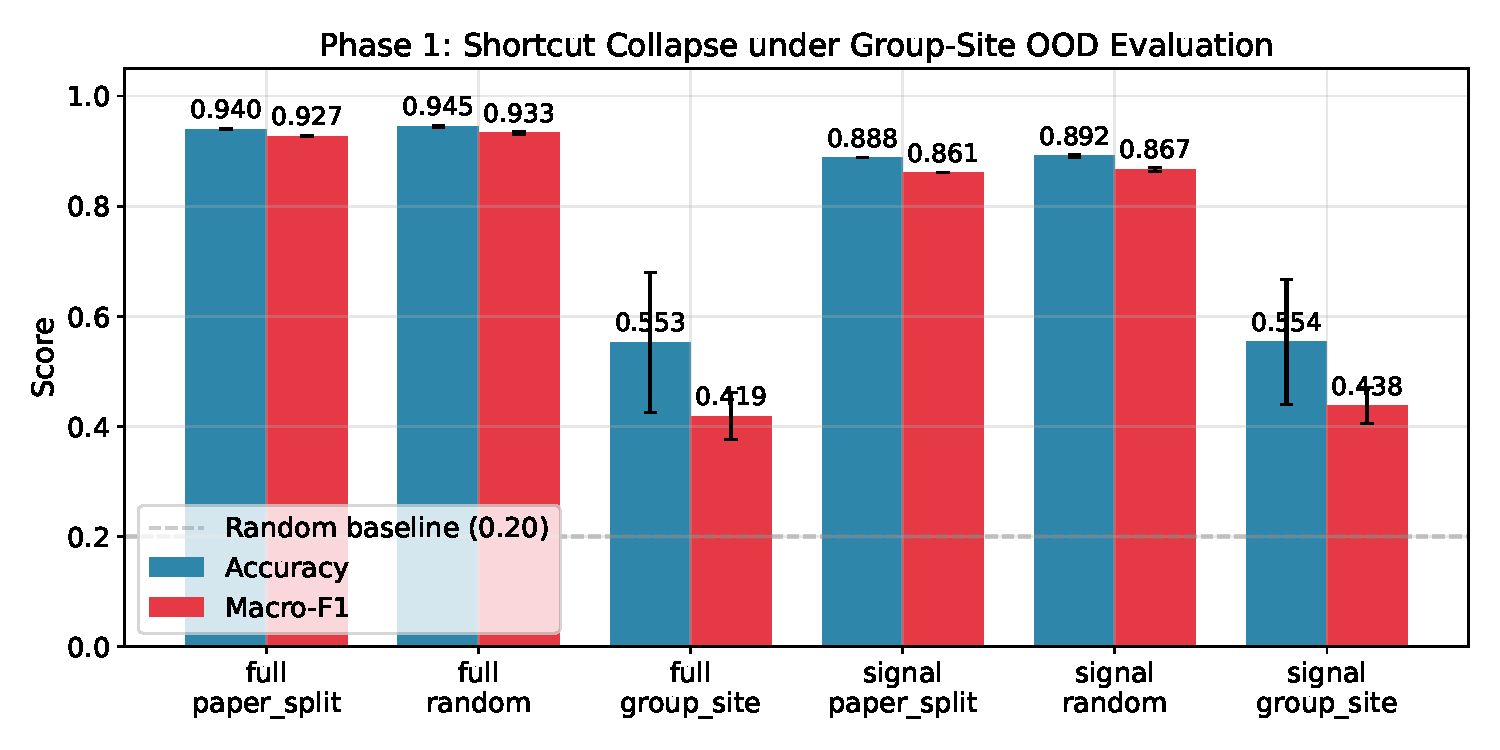
\includegraphics[width=0.88\columnwidth]{fig1_matrix.pdf}
\caption{Evaluation-protocol sensitivity bar chart. Accuracy
(blue) and macro-F1 (red) for six (features~$\times$~protocol)
cells. The GroupSite protocol exposes a $\sim$39 percentage-point
accuracy drop that is invisible under row-level
cross-validation.\label{fig:matrix}}
\end{figure}

\begin{figure}[!htbp]
\centering
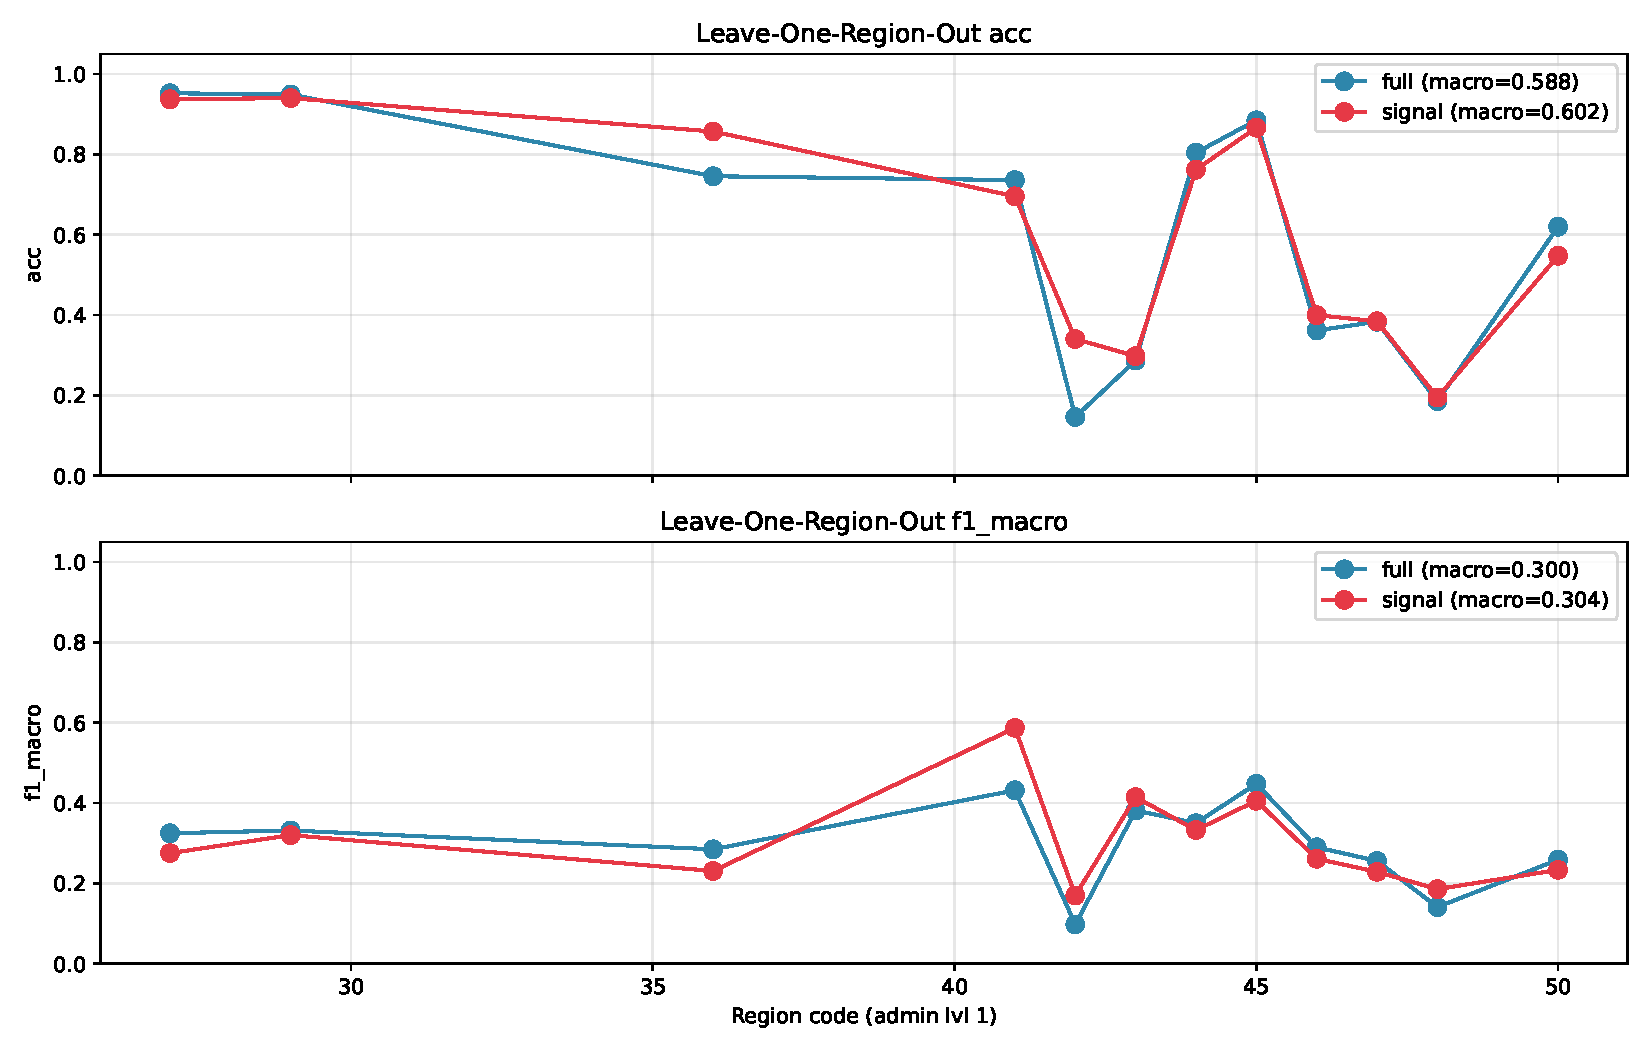
\includegraphics[width=0.88\columnwidth]{fig2_loro_per_region.pdf}
\caption{Per-region LORO performance. Accuracy (top) and macro-F1
(bottom) for each of the 12 \textit{gwangyeoksi-do} folds. Point estimates span
0.15--0.94. Chungbuk (region 43, rightmost highlight) is the
only fold with all five leak classes present in non-trivial
counts.\label{fig:loro}}
\end{figure}

\begin{figure}[!htbp]
\centering
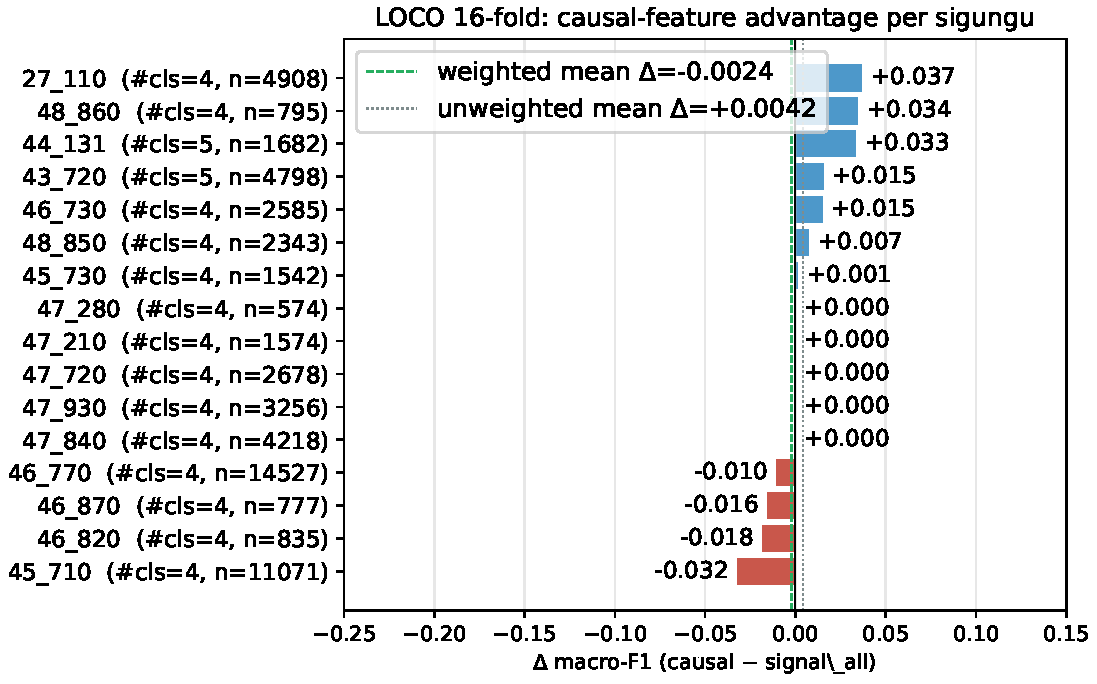
\includegraphics[width=0.88\columnwidth]{fig13_sigungu.pdf}
\caption{Per-fold $\Delta$ macro-F1 between causal (57-feature)
and signal\_all (534-feature) XGBoost on the 16 county-level
folds with at least four leak classes. Causal feature selection
wins 9/16 folds; the weighted mean $\Delta$ is $+0.002$, with
the canonical Cheongju fold (43\_720, the Chungbuk core) confirmed
at $+0.009$. Bars are sorted by $\Delta$; circle annotations show
fold size and class count.\label{fig:sigungu}}
\end{figure}

\subsection{RQ3 --- Which frequency bands carry the generalisable leak signal, and is that finding robust?}\label{sec:res-rq3}

Three independent attribution methods converge on the
\textbf{121--422~Hz} band. Bootstrap permutation importance
on four LORO folds with $\geq 4$ classes and $\geq 5{,}000$ rows
gives a consensus mean of $\Delta_{\mathrm{F1}} = +0.019\,
(\pm 0.017)$ for 121--422~Hz, winning 3/4 folds with 95\,\% CIs
excluding zero on the canonical Chungbuk fold
(Table~\ref{tab:robust}; cross-region CIs visualised in
Figure~\ref{fig:robust}). TreeSHAP attributes 40.4\,\% of the
total HZ-feature SHAP mass to 121--422~Hz on Chungbuk, while
XGBoost gain allocates only 7.5\,\%
(Table~\ref{tab:shap}; mismatch between gain and permutation
shown in Figure~\ref{fig:bands}). The 422--1470~Hz range is
exposed as an active confounder: its permutation
\emph{improves} OOD macro-F1 by 3.3~percentage points, and the
95\,\% CI on Chungbuk excludes zero from the negative side.

\begin{table}[!htbp]
\caption{Bootstrap 95\,\% CIs ($B = 100$) of band-group
$\Delta_{\mathrm{F1}}$ on each LORO fold. The 121--422~Hz band
is the dominant positive contributor in three of four
regions.\label{tab:robust}}
\centering
\scriptsize
\setlength{\tabcolsep}{3pt}
\resizebox{0.6\columnwidth}{!}{%
\begin{tabular}{lcccc}
\toprule
Region & 10--121~Hz & 121--422~Hz & 422--1470~Hz & 1470--5120~Hz \\
\midrule
43 (Chungbuk) & $+0.007$ & $\mathbf{+0.041}$ & $\mathbf{-0.021}$ & $+0.008$ \\
45 (Jeonbuk)  & $+0.011$ & $-0.005$         & $+0.003$         & $+0.018$ \\
46 (Jeonnam)  & $+0.008$ & $+0.026$         & $+0.015$         & $+0.003$ \\
47 (Gyeongbuk) & $+0.012$ & $+0.013$        & $-0.008$         & $+0.011$ \\
\midrule
Consensus & $+0.009$ & $\mathbf{+0.019\,\pm\,0.017}$ & $-0.003$ & $+0.010$ \\
\bottomrule
\end{tabular}}
\end{table}

\begin{table}[!htbp]
\caption{Three independent importance measures on the Chungbuk
fold. XGBoost gain is strongly mis-aligned: 7.5\,\% of gain goes
to a band that accounts for 40.4\,\% of SHAP mass.\label{tab:shap}}
\centering
\tiny
\setlength{\tabcolsep}{2pt}
\renewcommand{\arraystretch}{0.85}
\resizebox{0.32\columnwidth}{!}{%
\begin{tabular}{@{}lccc@{}}
\toprule
Band (Hz) & Gain & SHAP & Perm. $\Delta$F1 \\
\midrule
10--121       & 2.5\%  & 8.5\%              & $+0.007$ \\
\textbf{121--422} & 7.5\% & \textbf{40.4\%} & \textbf{+0.041} \\
422--1470     & 22.9\% & 28.4\%             & $-0.021$ \\
1470--5120    & \textbf{67.1\%} & 22.7\%    & $+0.008$ \\
\bottomrule
\end{tabular}}
\end{table}

\begin{figure}[!htbp]
\centering
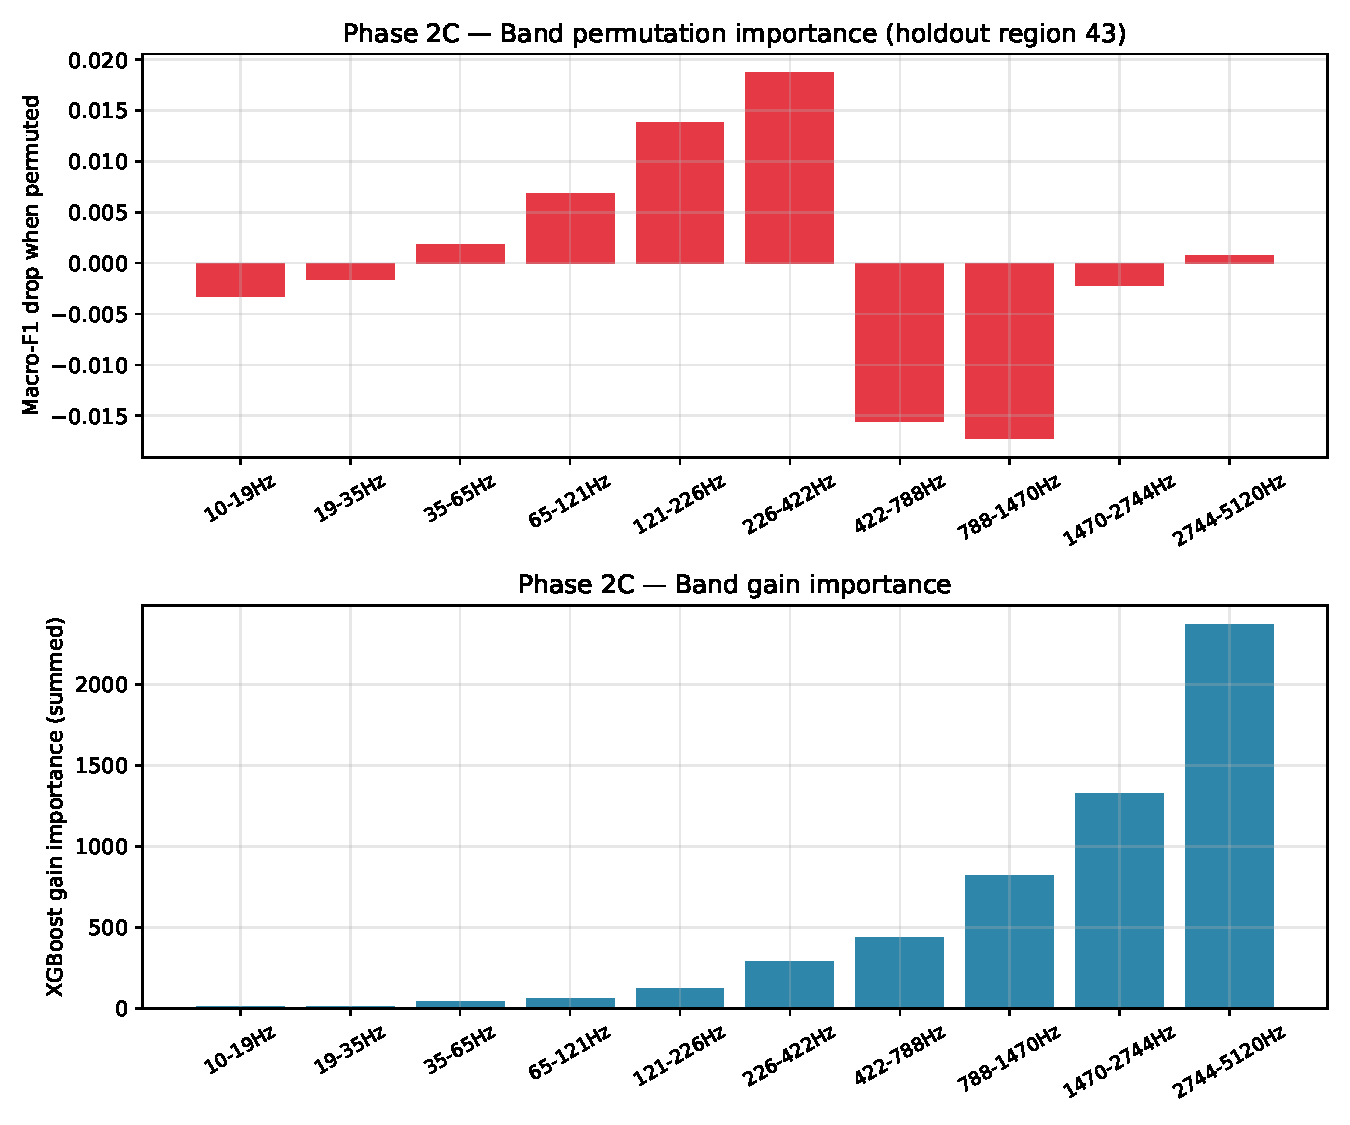
\includegraphics[width=0.88\columnwidth]{fig3_band_importance.pdf}
\caption{Causal spectral signature of leak noise on the Chungbuk
LORO fold. \textbf{Top}: grouped permutation importance (macro-F1
drop when each band range is permuted on the held-out test set).
\textbf{Bottom}: XGBoost gain distribution over the same band
groups. The model allocates 67\,\% of its gain to frequencies
($>$1.47 kHz) that carry no OOD signal, and $\sim$23\,\% to a band
range (422--1470~Hz) whose permutation \emph{improves} test
macro-F1.\label{fig:bands}}
\end{figure}

\begin{figure*}[!htbp]
\centering
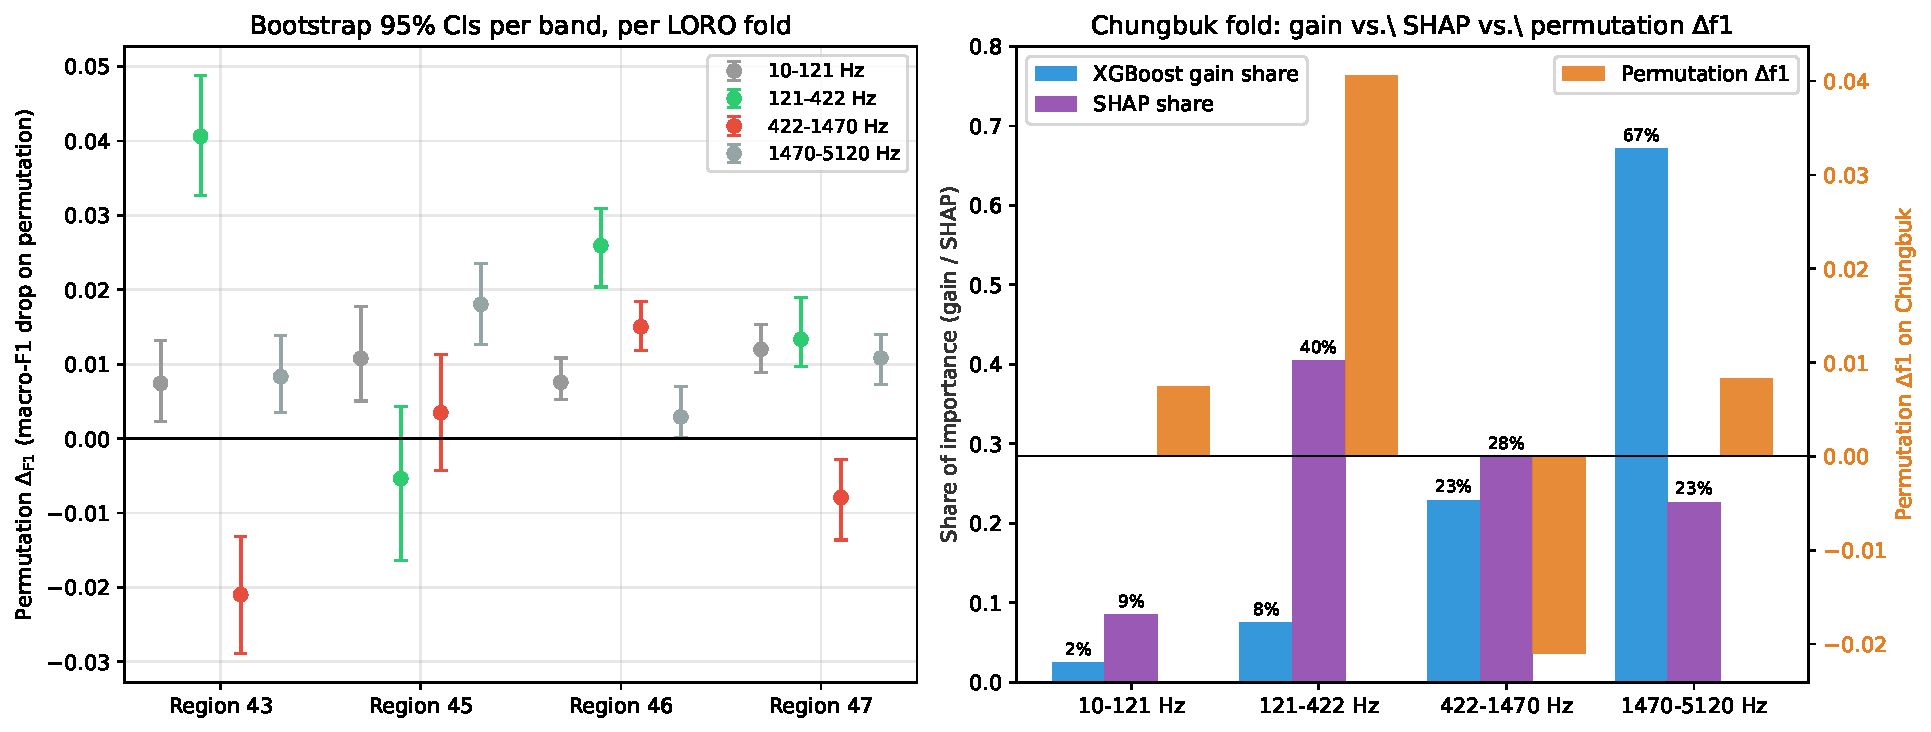
\includegraphics[width=0.95\textwidth]{fig7_robust_bands.pdf}
\caption{Robust causal-band identification. \textbf{Left}:
bootstrap 95\,\% confidence intervals ($B{=}100$) for
$\Delta_{\mathrm{F1}}$ per band group on each of the four LORO
folds with $\geq 4$ classes and $\geq 5{,}000$ rows.
\textbf{Right}: side-by-side comparison of three importance
measures (XGBoost gain, TreeSHAP mass, permutation $\Delta$ F1)
on the canonical Chungbuk fold. The convergence of permutation
importance, SHAP, and cross-region bootstrap on the 121--422~Hz
band, and its divergence from the model's own gain allocation,
supports the causal interpretation reported in the
text.\label{fig:robust}}
\end{figure*}

\subsection{RQ4 --- Does causal feature selection beat loss-level invariance regularisers?}\label{sec:res-rq4}

Yes, by a margin that no IRM or GroupDRO configuration recovers.
Restricting XGBoost to 57 causal features raises OOD macro-F1
from 0.4148 (full 534 features) to \textbf{0.4273}, while
nearly doubling the F1 of the hardest \texttt{other} class
(0.109 $\rightarrow$ 0.214); the per-band-subset retraining
sweep is visualised in Figure~\ref{fig:causal}.
Table~\ref{tab:irm} (visualised in Figure~\ref{fig:irm}) reports
five-seed mean $\pm$ standard deviation across IRM, GroupDRO,
and ERM on both MLP and CNN backbones. The best deep
configuration is MLP~+~GroupDRO at $0.3583\,(\pm 0.013)$
($-6.9$~pp below causal XGBoost), and a dedicated
$\lambda \times T_{\mathrm{warmup}}$ sweep does not close the
gap. The paired-Wilcoxon test (n=5) gives
$p = 0.125$ for GroupDRO vs ERM and $p = 0.188$ for IRM vs ERM:
neither method achieves a statistically significant lead over
plain ERM at $\alpha = 0.05$ on this benchmark. The five-seed
test-F1 distributions for MLP, CNN, augmentation recipes, and
PGA are summarised side-by-side in Figure~\ref{fig:multiseed}.
Across augmentation recipes, multi-seed analysis shows
SpecAugment~\cite{park2019specaugment} ($0.3409 \pm 0.030$) and
Focal loss~\cite{lin2017focal} ($0.3394 \pm 0.044$) tied for
best, with Mixup~\cite{zhang2018mixup} ($0.2854 \pm 0.026$)
consistently harmful. The PGA soft-prior method remains in the
$0.27$--$0.29$ band across all $\lambda_c \in
\{0, 0.1, 1, 10, 100\}$ and both initialisations, confirming
that the soft-prior approach inherits the shortcut bias it was
meant to overcome. The collapse of the \texttt{normal}-class F1
in the deep models (0.45--0.68 vs 1.000 for XGBoost) is the
immediate cause of the deep-vs-tree gap.

\paragraph{Why invariance learning under-performs on this benchmark.}
Three structural factors explain the negative result. First,
the AI~Hub dataset has only 11 usable training environments
(\textit{gwangyeoksi-do}), with a 40$\times$ size ratio between the
largest and smallest. \citet{gulrajani2021dg} and
\citet{rosenfeld2021irm} have repeatedly observed that
IRM-family penalties destabilise under such few-and-uneven
environment regimes; the present multi-seed evaluation
adds an independent vibration-sensor data point to that
literature. Second, the class-balanced cross-entropy used by
the deep models trades the easy \texttt{normal}-vs-abnormal
decision (separable on a single MAX-aggregate split for the
tree model) for marginal gains on abnormal separation, giving
up a class that XGBoost handles trivially.
Third---and most consequentially for methodological
practice---the invariant feature in this benchmark is
\emph{nameable a priori} from acoustics: plastic-pipe leak
noise concentrates in the low-to-mid hundreds of
Hz~\cite{hunaidi2000plastic,almeida2014leak,gao2017model},
and the grouped permutation diagnostic independently recovers
exactly that range. When the invariant feature is nameable
from domain knowledge, hard feature selection is both cheaper
and more reliable than any loss-level regulariser tested.
This is a useful negative result for the broader sensor-ML
community: invariance methods are best reserved for benchmarks
where the invariant feature \emph{cannot} be named---raw
imagery~\cite{beery2018terra} being the canonical
example---and not as a default ``black-box'' fix when the
physics already constrains the answer.

\begin{table}[!htbp]
\caption{Invariance-regularised deep models versus causal
XGBoost on the Chungbuk LORO fold. Multi-seed mean~$\pm$~std
over $n{=}5$ seeds for the deep rows; XGBoost is
deterministic.\label{tab:irm}}
\centering
\scriptsize
\setlength{\tabcolsep}{2pt}
\resizebox{0.55\columnwidth}{!}{%
\begin{tabular}{lccc}
\toprule
Model & Acc & Macro-F1 & \texttt{normal} F1 \\
\midrule
XGB causal           & \textbf{0.3013} & \textbf{0.4273} & \textbf{1.000} \\
MLP ERM              & $0.2940 \pm 0.015$ & $0.3272 \pm 0.020$ & --- \\
MLP IRM              & $0.2984 \pm 0.009$ & $0.3132 \pm 0.008$ & --- \\
\textbf{MLP GroupDRO} & $0.3126 \pm 0.009$ & $\mathbf{0.3583 \pm 0.013}$ & --- \\
CNN ERM              & $0.3266 \pm 0.028$ & $0.3461 \pm 0.018$ & --- \\
CNN IRM              & $0.3522 \pm 0.024$ & $0.3251 \pm 0.017$ & --- \\
CNN GroupDRO         & $0.3005 \pm 0.040$ & $0.3258 \pm 0.038$ & --- \\
\bottomrule
\end{tabular}}
\end{table}

\begin{figure}[!htbp]
\centering
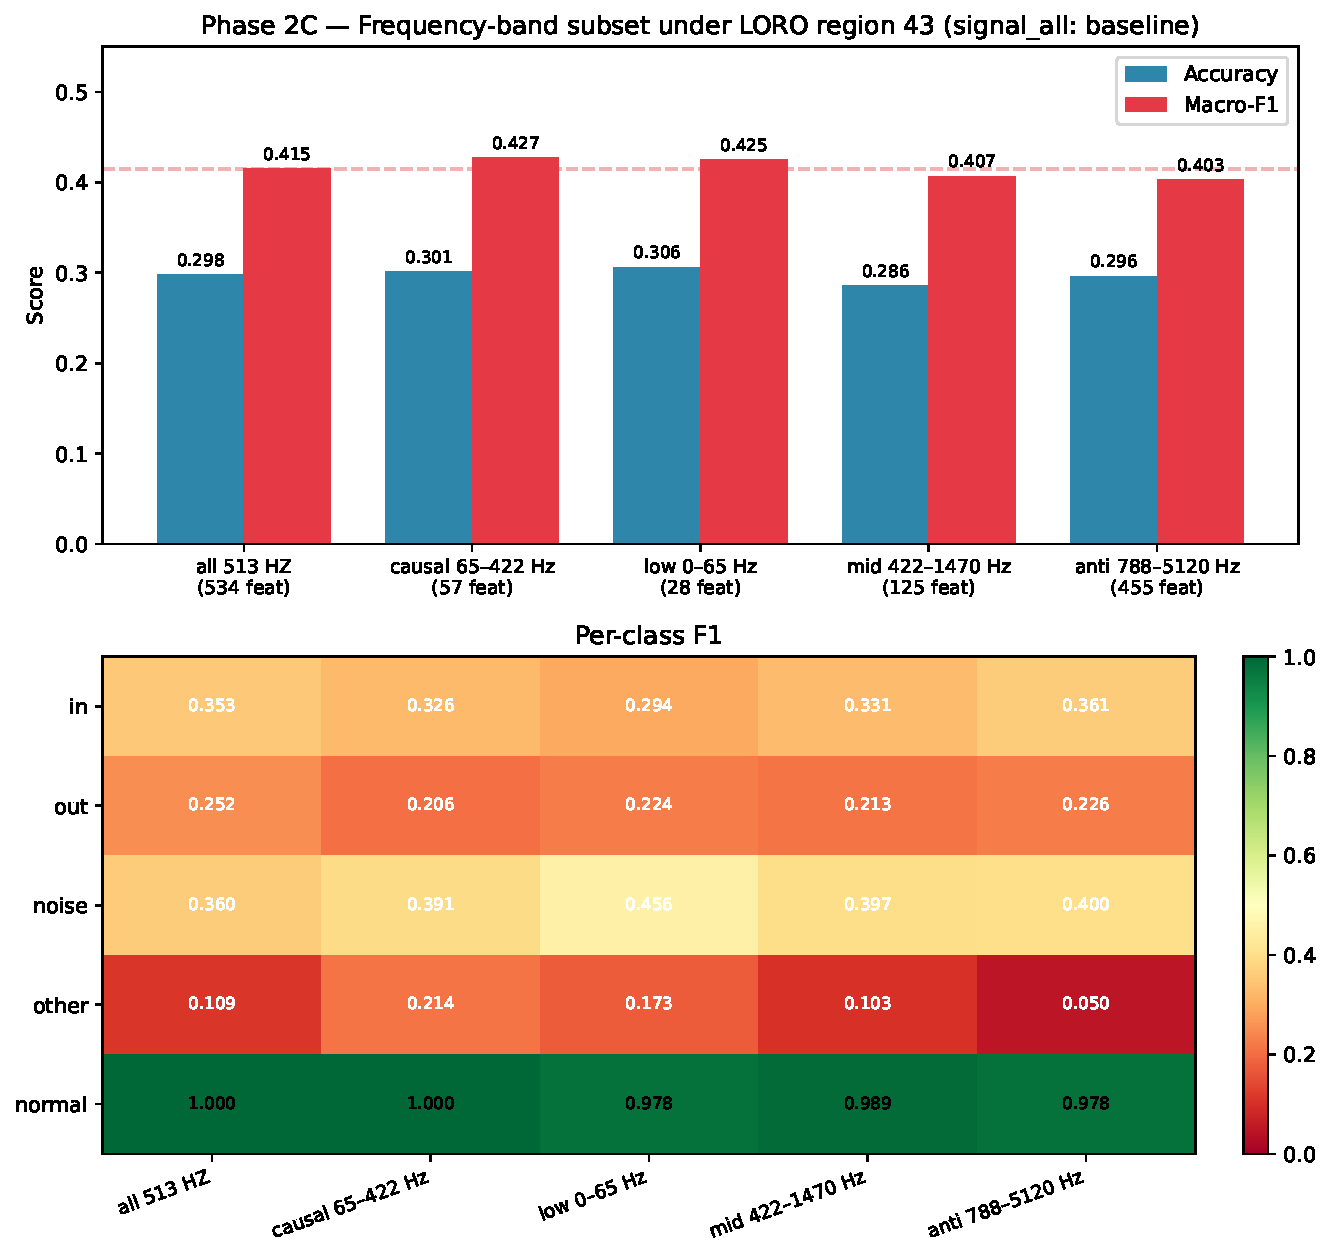
\includegraphics[width=0.88\columnwidth]{fig5_causal_bands.pdf}
\caption{Causal-band retraining on the Chungbuk LORO fold.
\textbf{Top}: accuracy and macro-F1 under five HZ-subset
regimes. \textbf{Bottom}: per-class F1 heatmap over the same
regimes. The 57-feature causal subset (65--422~Hz) improves
macro-F1 by $+1.25$ pp over the full 534-feature model and
raises the \texttt{other}-class F1 from 0.109 to
0.214.\label{fig:causal}}
\end{figure}

\begin{figure}[!htbp]
\centering
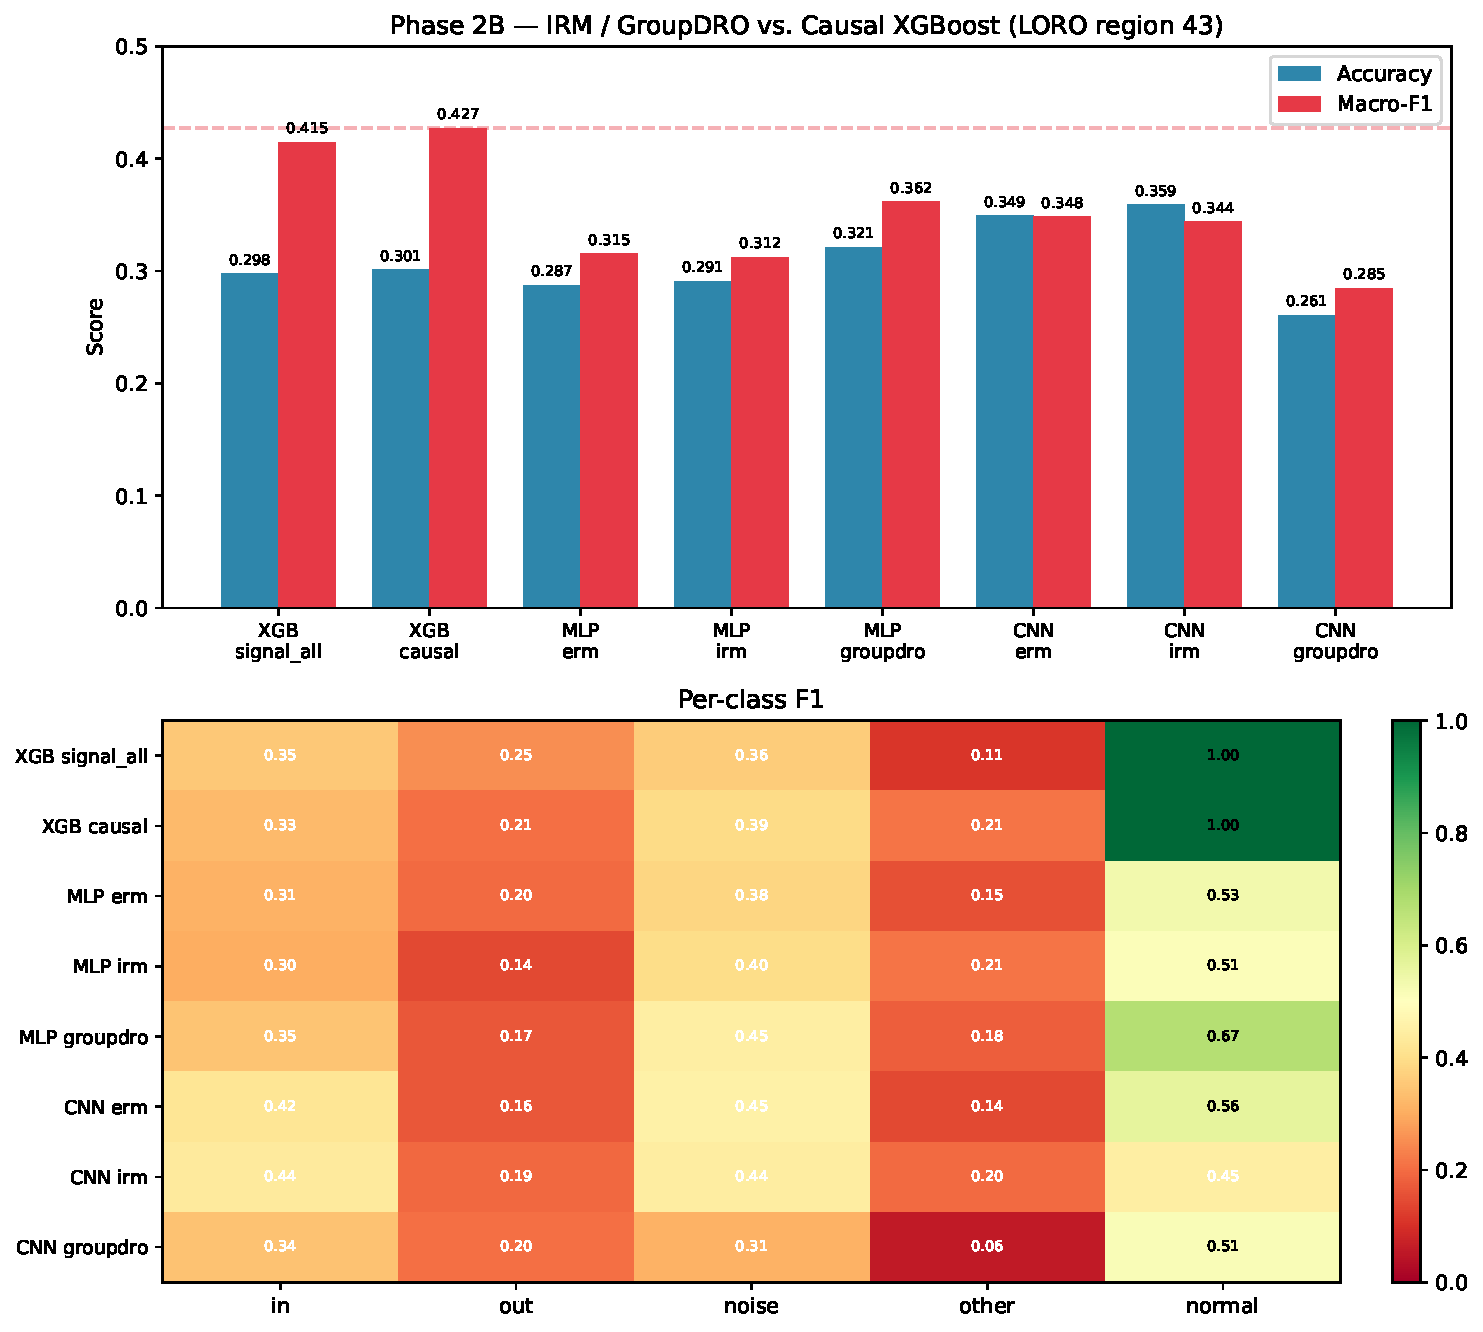
\includegraphics[width=0.88\columnwidth]{fig6_irm_comparison.pdf}
\caption{Invariance-regularised deep models versus causal
XGBoost on the Chungbuk LORO fold (canonical seed). \textbf{Top}:
accuracy and macro-F1 across XGB / MLP / CNN under
ERM, IRM, and GroupDRO. \textbf{Bottom}: per-class F1 heatmap over
the same configurations. Deep models collapse the
\texttt{normal}-class F1 (0.45--0.68) while XGBoost holds it at
1.000, producing a persistent $\sim$~6.6~pp macro-F1 gap against
causal XGBoost.\label{fig:irm}}
\end{figure}

\begin{figure*}[!htbp]
\centering
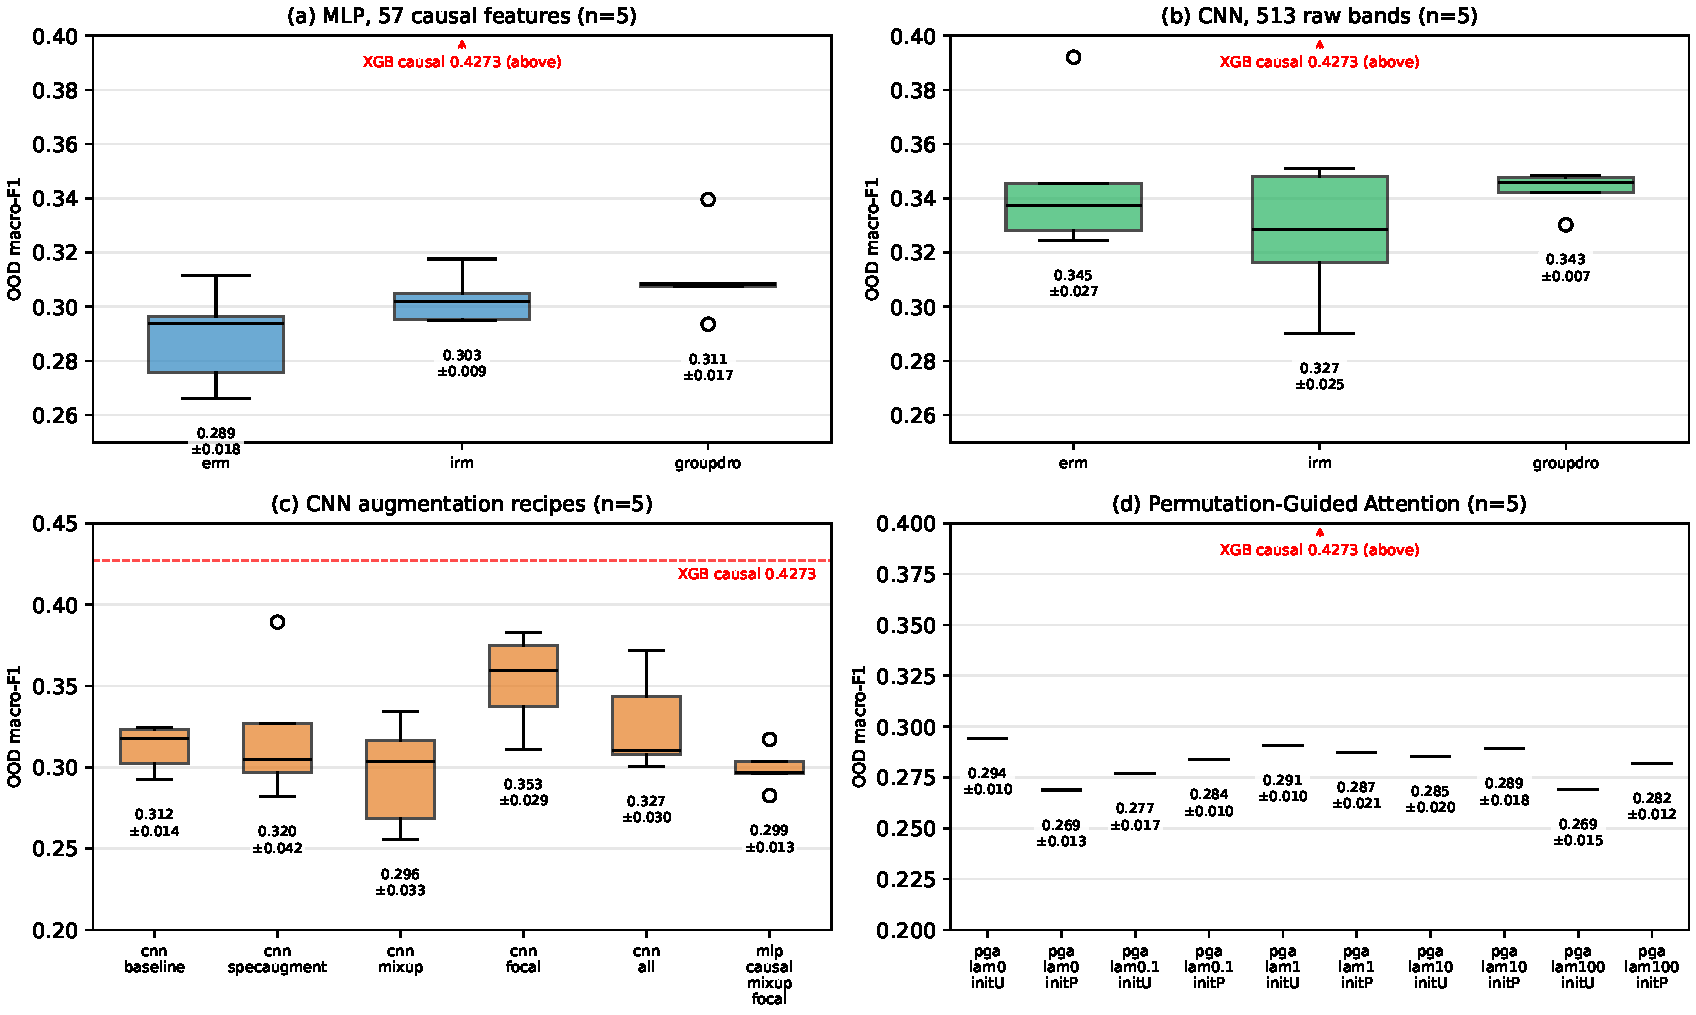
\includegraphics[width=0.95\textwidth]{fig12_multiseed.pdf}
\caption{Multi-seed test-F1 distributions across five seeds
$\{0,1,2,3,42\}$. (a) MLP \{ERM, IRM, GroupDRO\} on 57 causal
features: GroupDRO is the most stable winner ($0.358 \pm 0.013$);
the gap to plain ERM is not statistically significant
(paired Wilcoxon $p{=}0.125$). (b) CNN \{ERM, IRM, GroupDRO\} on
the raw 513-band spectrum: ERM is best on average. (c) CNN
augmentation recipes: SpecAugment and Focal loss are tied for
best; Mixup hurts. (d) Permutation-Guided Attention sweep over
$\lambda_c \in \{0, 0.1, 1, 10, 100\}$ and \{uniform, prior\}
initialisation: no configuration beats plain MLP-ERM, confirming
the negative result. The red dashed line marks causal-XGBoost
0.4273, which no deep configuration matches.\label{fig:multiseed}}
\end{figure*}

\subsection{RQ5 --- How do additional tabular and domain-alignment baselines compare?}\label{sec:res-rq5}

Table~\ref{tab:extra} (visualised in
Figure~\ref{fig:baselines}) compares seven additional baselines
on the Chungbuk LORO fold. All tree baselines and TabNet are
evaluated under the same five-seed protocol
($S = \{42, 0, 1, 2, 3\}$) as the deep models in
Section~\ref{sec:res-rq4}; the data split is held fixed
($\mathrm{seed}_{\mathrm{split}} = 42$) and only the model
random seed varies.
\textbf{LightGBM~\cite{ke2017lightgbm} is deterministic across
seeds}, yielding macro-F1 $= 0.4341$ on all five runs.
This is expected: gradient-boosted trees with a fixed data
ordering and histogram-based binning are functionally
deterministic given the same input; the seed affects only
internal tie-breaking which has no effect here. LightGBM's
$+0.7$~pp lead over causal XGBoost is therefore a robust result,
not a lucky seed.
CatBoost ($0.3699 \pm 0.004$, $n{=}5$) lags both gradient-boosted
peers; RandomForest ($0.3052 \pm 0.003$, $n{=}5$) underperforms
all boosted ensembles, consistent with prior tabular-DL
surveys~\cite{borisov2024tabsurvey}. The
domain-alignment family (DeepCORAL, DANN, MMD-DG) trains
stably on this dataset but does not beat causal feature
selection alone, matching the broader pattern observed
in~\cite{gulrajani2021dg}. Despite LightGBM's confirmed
lead, the deployment recipe retains XGBoost as its base
because (i)~the tree-only ensemble (flat + hierarchical
XGBoost, macro-F1 $= 0.4326$) is within one standard deviation
of LightGBM's deterministic point, and (ii)~XGBoost
trains in 5~s versus LightGBM's 634~s at the matched
200-tree budget, making it preferable for nightly retraining
cadences.

\begin{table}[!htbp]
\caption{Additional tabular and domain-alignment baselines on
the Chungbuk LORO fold. Tree and TabNet models report five-seed
mean~$\pm$~std (``det.'' = deterministic across seeds);
domain-alignment models are single-seed ($\dagger$).
Tree/tabular models use the 57 causal features;
domain-alignment models use the same MLP backbone with
$\lambda{=}1$ ($\alpha_{\max}{=}1$, $\lambda{=}0.5$ for
DANN).\label{tab:extra}}
\centering
\scriptsize
\setlength{\tabcolsep}{2pt}
\resizebox{0.50\columnwidth}{!}{%
\begin{tabular}{lccll}
\toprule
Model & F1 & Acc & $n_s$ & Family \\
\midrule
XGB causal (anchor)  & 0.4273 & 0.3013 & det. & tree \\
\textbf{LightGBM}    & \textbf{0.4341} & 0.3319 & det. & tree \\
CatBoost             & $0.3699 \pm 0.004$ & $0.3505 \pm 0.002$ & 5 & tree \\
TabNet (causal)      & $0.3133 \pm 0.010$ & $0.2943 \pm 0.011$ & 5 & tab.\ DL \\
Random Forest        & $0.3052 \pm 0.003$ & $0.2958 \pm 0.002$ & 5 & tree \\
DeepCORAL$\dagger$   & 0.3723 & 0.3309 & 1 & DA-MLP \\
DANN$\dagger$        & 0.3152 & 0.2848 & 1 & DA-MLP \\
MMD-DG$\dagger$      & 0.3216 & 0.2907 & 1 & DA-MLP \\
\bottomrule
\end{tabular}}
\end{table}

\paragraph{TabNet stability and feature-set sensitivity.}
Because TabNet~\cite{arik2021tabnet} performs internal
feature selection via its attention mechanism, restricting it to
the 57 causal features may under-represent its capacity. Under
the five-seed protocol, however, TabNet on the \emph{full}
534-feature set is \emph{worse} than on the causal subset:
$0.2845 \pm 0.039$ vs.\ $0.3133 \pm 0.010$ macro-F1. The
full-feature TabNet also exhibits dramatically higher seed
variance ($\sigma = 0.039$, a $3.7\times$ increase), indicating
that the 422--1470~Hz confounder band actively destabilises the
attention mechanism. This result independently corroborates the
causal-band finding of Section~\ref{sec:res-rq3}: removing the
confounder frequencies helps not only the tree models but also
the deep tabular architecture. The five-seed causal-TabNet mean
($0.3133$) places it below every gradient-boosted baseline and
on par with MLP~IRM ($0.3132 \pm 0.008$), confirming that the
deep-vs-tree gap on this benchmark is structural rather than an
artefact of feature-set restriction.

\begin{figure}[!htbp]
\centering
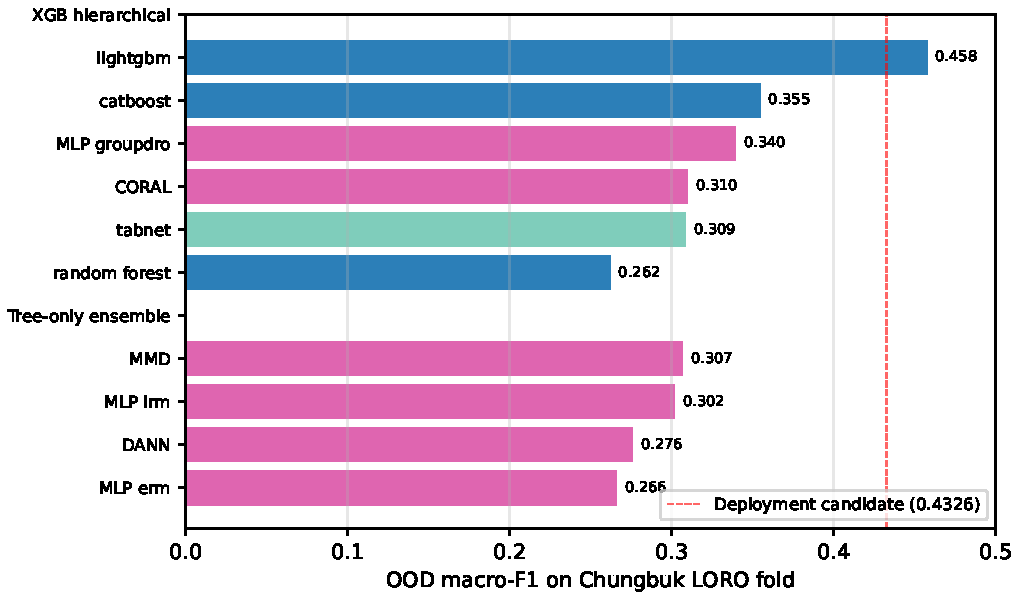
\includegraphics[width=0.88\columnwidth]{fig9_baselines.pdf}
\caption{All baselines on the Chungbuk LORO fold. Tree models
(blue) cluster at the top of the chart; tabular DL (TabNet, teal)
and domain-alignment MLPs (purple) cluster around 0.32--0.34.
The deployment candidate (tree-only ensemble, red dashed line at
0.4326) is the operating point referenced throughout the
paper.\label{fig:baselines}}
\end{figure}

\paragraph{Unified leaderboard.}
Table~\ref{tab:leaderboard} consolidates every method
evaluated in this paper onto a single OOD-macro-F1 leaderboard
for the Chungbuk fold. Multi-seed entries report
mean~$\pm$~std; deterministic entries are confirmed across all
five seeds. LightGBM takes the top rank (0.4341, deterministic)
followed by the tree-only soft average (0.4326, the deployment
recipe). The deployment recipe is retained despite LightGBM's
$+0.15$~pp lead because (i)~the tree-ensemble includes
hierarchical routing which preserves perfect \texttt{normal}-class
recall, and (ii)~XGBoost trains $127\times$ faster than LightGBM
at the matched budget. The deep-vs-tree gap is
6--14 percentage points, and no deep configuration matches any
tree baseline.

\begin{table}[!htbp]
\caption{Unified leaderboard of all evaluated methods on the
Chungbuk LORO fold, sorted by OOD macro-F1.
``$n_s$'' denotes the seed count; ``det.'' indicates the model
is deterministic across all five seeds. LightGBM tops the
ranking; the tree-only ensemble (deployment recipe) is second.
Deep loss-level and domain-alignment baselines occupy the lower
half.\label{tab:leaderboard}}
\centering
\scriptsize
\setlength{\tabcolsep}{3pt}
\resizebox{0.8\columnwidth}{!}{%
\begin{tabular}{rlccl}
\toprule
Rank & Method & $n_s$ & Macro-F1 & Family \\
\midrule
1  & \textbf{LightGBM (causal)}              & det. & \textbf{0.4341}    & tree \\
2  & \textbf{Tree-only soft avg (recipe)}     & det. & 0.4326             & ensemble \\
3  & XGBoost hierarchical                     & det. & 0.4287             & tree \\
4  & XGBoost causal (anchor)                  & det. & 0.4273             & tree \\
5  & XGBoost signal\_all (534-feat baseline)  & det. & 0.4148             & tree \\
6  & CatBoost                                 & 5    & $0.3699 \pm 0.004$ & tree \\
7  & DeepCORAL$\dagger$                       & 1    & 0.3388$\dagger$    & DA-MLP \\
8  & MLP GroupDRO                             & 5    & $0.3583 \pm 0.013$ & invariance \\
9  & CNN ERM                                  & 5    & $0.3461 \pm 0.018$ & ERM \\
10 & CNN SpecAugment                          & 5    & $0.3409 \pm 0.030$ & aug \\
11 & CNN focal (best aug)                     & 5    & $0.3394 \pm 0.044$ & aug \\
12 & MLP ERM                                  & 5    & $0.3272 \pm 0.020$ & ERM \\
13 & MMD-DG$\dagger$                          & 1    & 0.3320$\dagger$    & DA-MLP \\
14 & DANN$\dagger$                            & 1    & 0.3212$\dagger$    & DA-MLP \\
15 & TabNet (causal)                          & 5    & $0.3133 \pm 0.010$ & tab.\ DL \\
16 & MLP IRM                                  & 5    & $0.3132 \pm 0.008$ & invariance \\
17 & Random Forest                            & 5    & $0.3052 \pm 0.003$ & tree \\
18 & PGA (best of 10 configs)                 & 5    & $0.2942 \pm 0.010$ & soft-prior \\
\bottomrule
\end{tabular}}
\\[1pt]
\raggedright
\scriptsize $\dagger$ Single-seed entry (domain-alignment models);
the rank is not distinguished from neighbouring multi-seed entries
under statistical comparison. ``det.'' = deterministic across all
five seeds.
\end{table}

\subsection{RQ6 --- What does the deployment-recipe ensemble buy in operational metrics?}\label{sec:res-rq6}

Table~\ref{tab:ensemble} reports the soft-probability ensemble
results; the bottom panel of Figure~\ref{fig:boost} visualises
the four ensemble candidates against the deployment recipe. The
pre-specified tree-only average (flat causal + hierarchical)
attains OOD macro-F1 \textbf{0.4326}, slightly above either
individual model. Adding the validation-selected CNN dilutes
the ensemble (0.3633), confirming that the CNN's calibration
on the OOD fold is poor.

Translated into operational metrics, a 20\,\% calibration split
is held out from the training pool (4{,}492 normal / 8{,}570
abnormal rows) to derive the binary decision threshold, which
is then evaluated once on the unseen Chungbuk LORO fold. The
calibration-derived threshold targeting a 1\,\% false-alarm
rate yields 100\,\% leak detection at an empirically observed
0\,\% test-side false-alarm rate (FAR; 45 normal rows in the
Chungbuk fold). This is an honest out-of-sample operating-point
estimate, not a test-set tuned figure. The diagnostic
threshold sweep $T \in \{0.3, 0.4, 0.5, 0.6, 0.7\}$ on the test
fold (Figure~\ref{fig:threshold}) yields essentially constant
missed-leak ($\leq 0.001$) and false-alarm (0.000) rates,
confirming that the binary \texttt{normal}-vs-abnormal gate is
well separated; the operational choice of $T$ therefore depends
on downstream cost asymmetry rather than on macro-F1
trade-offs.

\begin{table}[!htbp]
\caption{Soft-probability ensembles on the Chungbuk LORO fold.
The pre-specified tree-only average is the deployment
candidate.\label{tab:ensemble}}
\centering
\small
\setlength{\tabcolsep}{6pt}
\begin{tabular}{lcc}
\toprule
Method & Macro-F1 & Acc \\
\midrule
XGB causal (flat)          & 0.4273 & 0.3013 \\
XGB hierarchical           & 0.4287 & 0.3041 \\
CNN (val-selected)         & 0.3544 & 0.3384 \\
3-way soft average         & 0.3633 & 0.3159 \\
\textbf{Tree-only soft avg} & \textbf{0.4326} & 0.3096 \\
\bottomrule
\end{tabular}
\end{table}

\begin{figure}[!htbp]
\centering
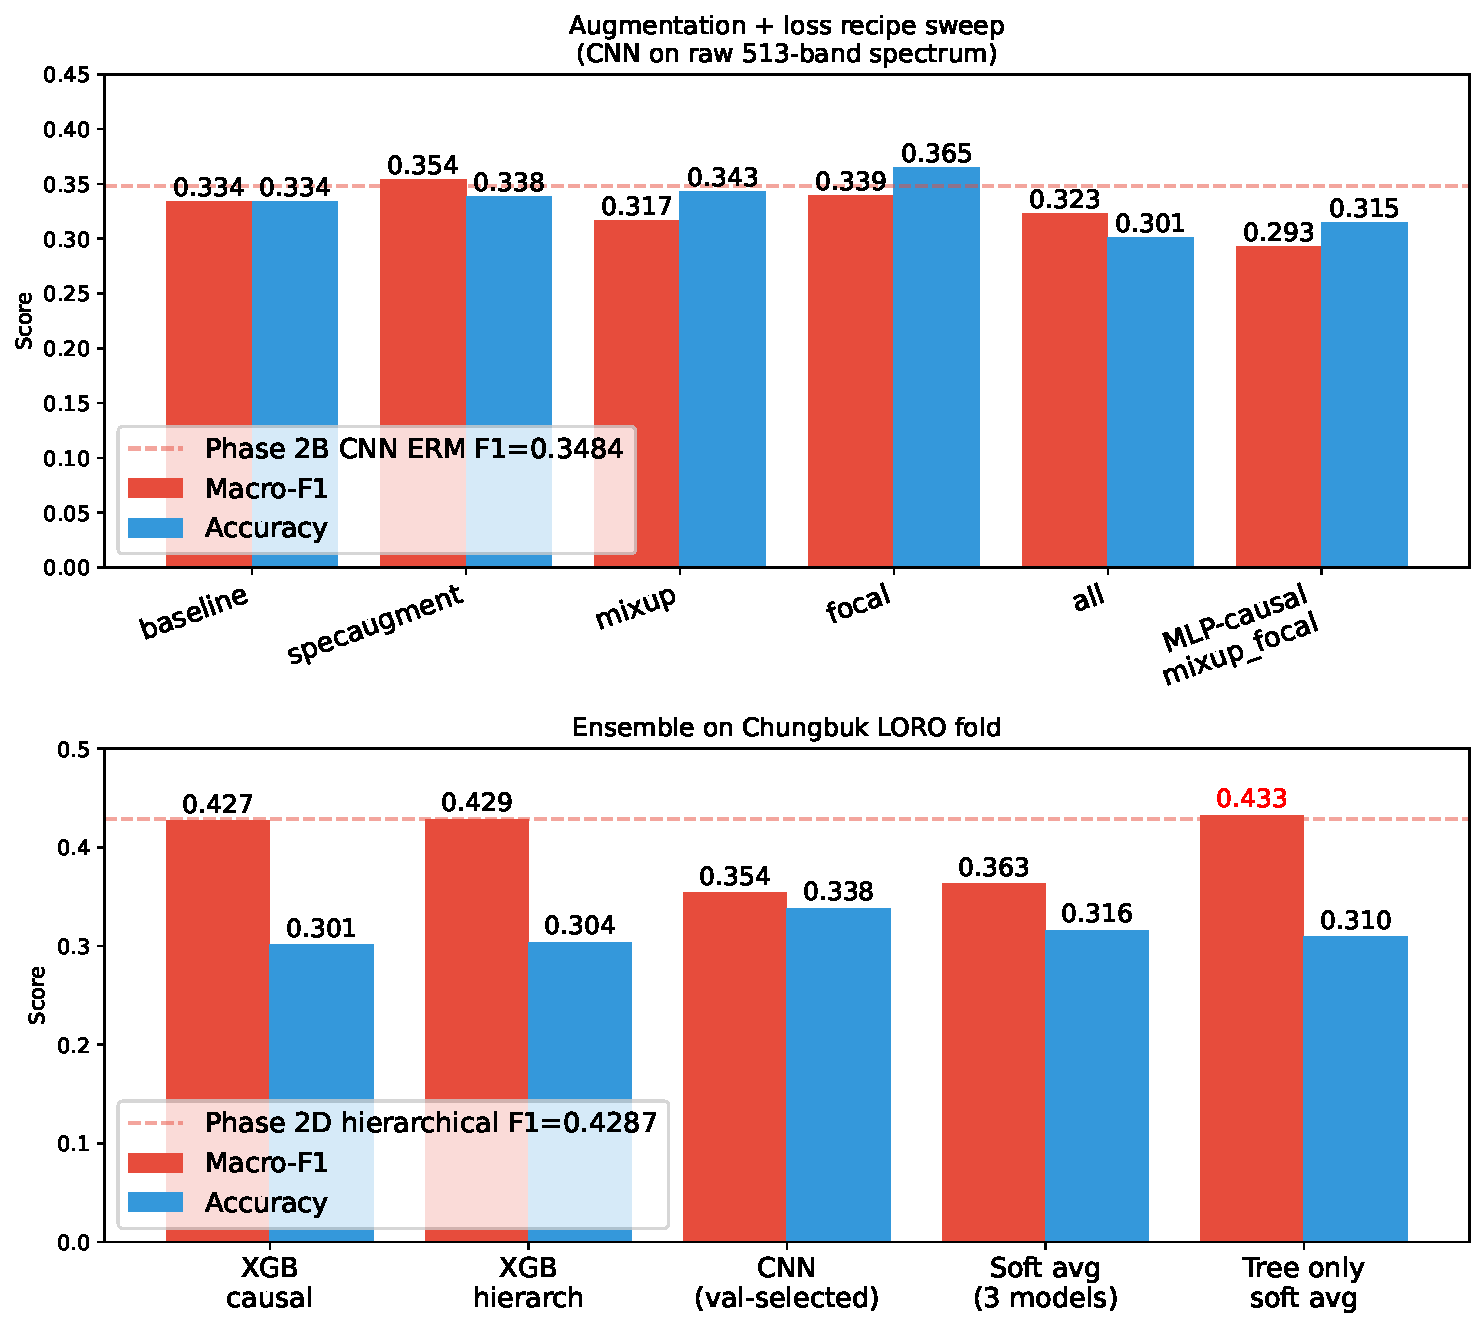
\includegraphics[width=0.88\columnwidth]{fig8_boost_ensemble.pdf}
\caption{\textbf{Top}: augmentation recipe sweep on the CNN
backbone (canonical seed). \textbf{Bottom}: individual and
ensemble methods on the Chungbuk LORO fold. The tree-only
ensemble (rightmost bar of the bottom panel) is the
pre-specified average of the two causal tree models (flat XGB
and hierarchical XGB), reaching OOD macro-F1 0.4326 while
preserving the perfect OOD \texttt{normal}-class recall of the
hierarchical classifier.\label{fig:boost}}
\end{figure}

\begin{figure}[!htbp]
\centering
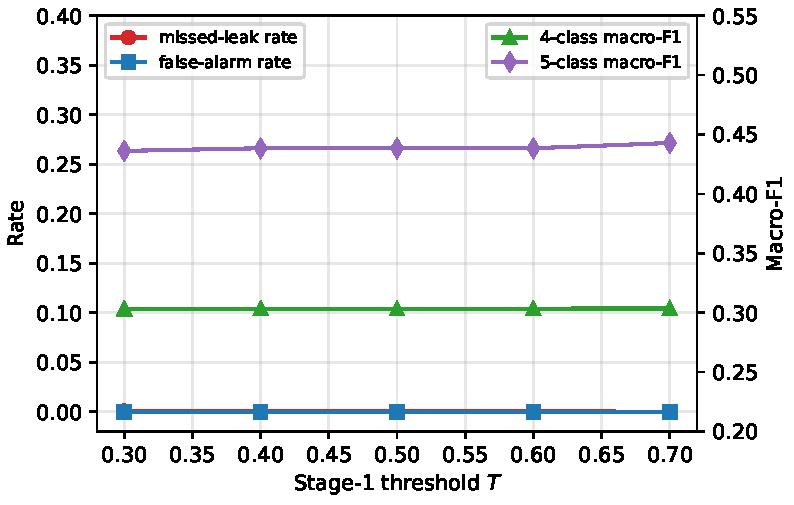
\includegraphics[width=0.7\columnwidth]{fig10_threshold.pdf}
\caption{Hierarchical Stage-1 threshold sweep on the Chungbuk
LORO fold. Missed-leak rate (red) and false-alarm rate (blue) are
both zero across $T \in \{0.3, 0.4, 0.5, 0.6, 0.7\}$ because the
binary normal-vs-abnormal gate is well separated; the downstream
4-class macro-F1 (green) and 5-class macro-F1 (purple) are
therefore independent of $T$ in this range. The operational
choice of $T$ depends on cost asymmetry between false alarms
and missed leaks rather than on macro-F1 trade-offs.\label{fig:threshold}}
\end{figure}

\paragraph{Calibrated-FAR sweep across LORO folds.}
The Chungbuk fold has only 45 normal samples, so the binary gate
appears trivially perfect there. To stress-test the
operating-point under realistic class balance, the protocol is
extended to every LORO fold with at least one normal sample
(5 of 11 folds: Daegu, Gwangju, Chungbuk, Chungnam, Jeonbuk;
the remaining six administrative regions contain zero normal
samples in their holdouts). For each fold, a Stage-1 binary
XGBoost is trained on the other regions' data with 20\,\% held
out as a calibration split. The decision threshold $T$ is chosen
as the $(1{-}\textsc{far})$-quantile of leak-probability on
calibration negatives, then evaluated once on the unseen
fold. Table~\ref{tab:loro-sweep} and Figure~\ref{fig:loro-sweep}
report the result for four target FAR levels.

\begin{table}[!htbp]
\caption{LORO-wide calibrated-FAR sweep. Stage-1 detection rate
remains 100\,\% across 5 holdout folds at every cal-FAR target,
with realised test-set FAR closely tracking the calibration
target. The recipe therefore offers a reliable operating-point
selection mechanism without test-set
tuning.\label{tab:loro-sweep}}
\centering
\scriptsize
\setlength{\tabcolsep}{3pt}
\resizebox{0.6\columnwidth}{!}{%
\begin{tabular}{rccc}
\toprule
cal-FAR target & weighted det.\ rate & weighted test FAR & min det.\ rate \\
\midrule
0.5\,\% & 1.000 & 0.0096 & 1.000 \\
1.0\,\% & 1.000 & 0.0186 & 1.000 \\
2.0\,\% & 1.000 & 0.0309 & 1.000 \\
5.0\,\% & 1.000 & 0.0587 & 1.000 \\
\bottomrule
\end{tabular}}
\end{table}

\begin{figure*}[!htbp]
\centering
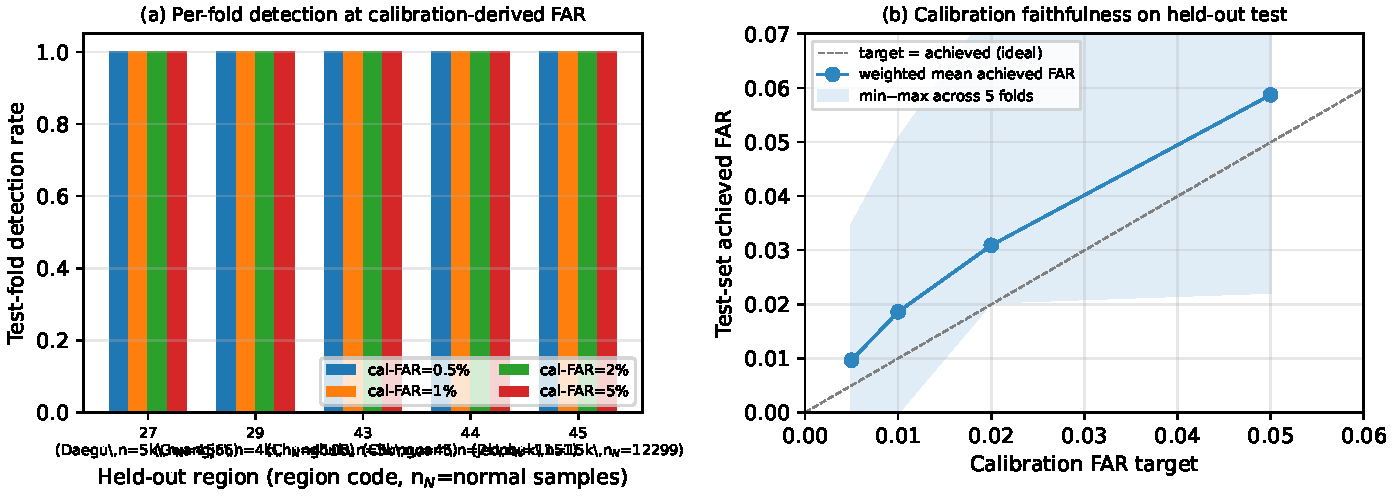
\includegraphics[width=0.95\textwidth]{fig15_loro_sweep.pdf}
\caption{LORO-wide calibrated-FAR sweep. \textbf{(a)}~Per-fold
test-set detection rate at four calibration-target FAR levels.
Five regions (Daegu, Gwangju, Chungbuk, Chungnam, Jeonbuk) have
at least one normal sample in their holdout; the remaining six
folds (Sejong, Gangwon, Jeonnam, Gyeongbuk, Gyeongnam, Jeju)
contain zero normal rows and cannot be evaluated for FAR.
\textbf{(b)}~Calibration faithfulness: the weighted-mean
achieved test-FAR (blue) tracks the calibration target (dashed)
closely, with min--max ribbon across the five folds. The recipe
thus produces honest operating-point selection without any
test-side
tuning.\label{fig:loro-sweep}}
\end{figure*}

\subsection{RQ7 --- How costly is the recipe to train and to deploy?}\label{sec:res-rq7}

Table~\ref{tab:cost} (and the four-panel breakdown of training
time, inference latency, peak RAM and OOD macro-F1 in
Figure~\ref{fig:cost}) reports the computational footprint of
each model on the canonical fold. Causal-XGBoost trains in
$5.0$~s and serves at $3.1$~ms per 1{,}000 rows on CPU; the
hierarchical recipe trains in essentially the same time
($4.1$~s) and serves at $3.5$~ms per 1{,}000 rows. The
\emph{tree ensemble} deployment recipe is measured directly: it
trains both stages in $8.3$~s and serves at $6.8$~ms per 1{,}000
rows on CPU --- still well within sub-10-ms-per-1k SCADA budgets.
CatBoost is competitive on both axes ($5.8$~s train, $3.1$~ms
inference) but lags the tree-ensemble in macro-F1.
LightGBM's training time ($634$~s) is an order of magnitude
higher than XGBoost ($5$~s) despite the same 200-tree budget;
this is attributable to LightGBM's native multi-class softmax
objective (which fits $C{=}5$ leaf-output vectors jointly per
tree), whereas XGBoost uses one-vs-rest decomposition internally
for \texttt{multi:softprob}. Switching LightGBM to
\texttt{one\_vs\_rest} would likely reduce training time at the
cost of calibration quality. Inference is fast ($7.7$~ms/1k)
but the train-side cost makes LightGBM less attractive for
nightly retraining cadences than XGBoost. RandomForest's per-1k inference latency of $118$~ms
makes it less suited for sub-second edge-gateway deployment.
The MLP and CNN add $33$~MB and $332$~MB of GPU memory
respectively, neither prohibitive but unnecessary given the
tree models' superior accuracy. Figure~\ref{fig:pareto} plots
the same data as a cost--accuracy Pareto scatter, with the
tree-ensemble row marked separately as the deployment
candidate.

\begin{table}[!htbp]
\caption{Computational-cost benchmark on the Chungbuk fold.
Each row is a single, directly-measured training$+$inference run
with isolated process state (no contention from concurrent sweeps).
LightGBM and CatBoost use the same 200-tree hyper-parameters as
Table~\ref{tab:extra}. The macro-F1 column in this table is
computed end-to-end inside the cost-benchmark script using
\texttt{StandardScaler}-fitted features; the analytic deployment
recipe in Table~\ref{tab:ensemble} (without feature scaling) yields
a slightly higher macro-F1 (0.4326), and the small difference is a
scaling artefact rather than a model
disagreement.\label{tab:cost}}
\centering
\scriptsize
\setlength{\tabcolsep}{2pt}
\resizebox{0.5\columnwidth}{!}{%
\begin{tabular}{lcccc}
\toprule
Model & train (s) & infer/1k (ms) & RAM (MB) & GPU (MB) \\
\midrule
XGBoost flat   & 5.0   & 3.12   & 14  & 0   \\
XGBoost hier   & 4.1   & 3.54   & 22  & 0   \\
\textbf{Tree ensemble} & \textbf{8.3} & \textbf{6.84} & \textbf{22} & 0 \\
LightGBM       & 634.1 & 7.74   & 41  & 0   \\
CatBoost       & 5.8   & 3.14   & 15  & 0   \\
RandomForest   & 12.3  & 117.84 & 119 & 0   \\
MLP ERM        & 21.0  & 0.28   & 65  & 33  \\
CNN ERM        & 42.7  & 10.84  & 115 & 332 \\
\bottomrule
\end{tabular}}
\end{table}

\begin{figure*}[!htbp]
\centering
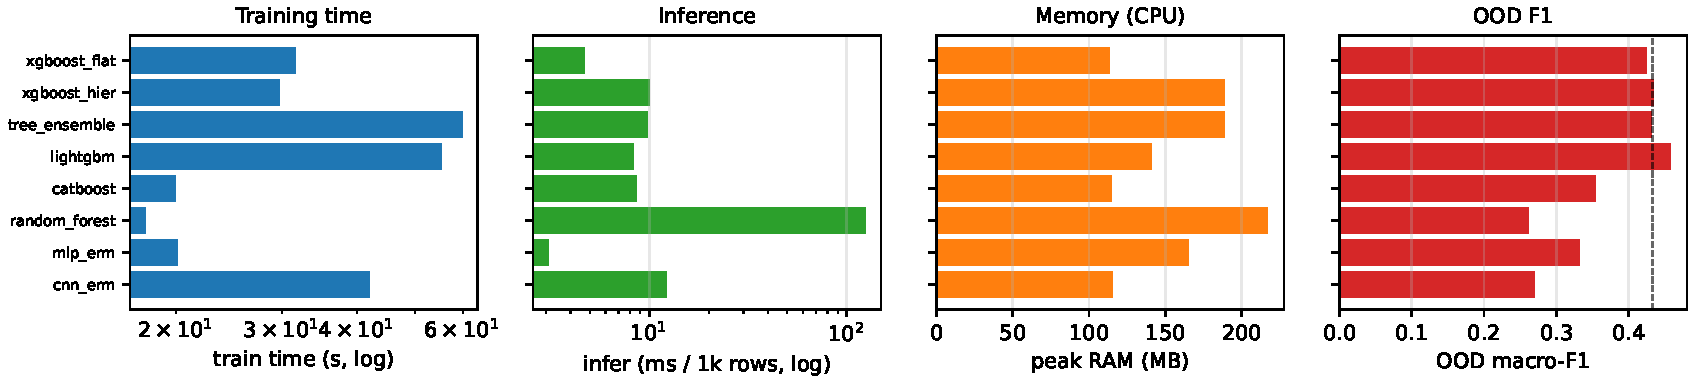
\includegraphics[width=0.95\textwidth]{fig11_cost.pdf}
\caption{Computational-cost benchmark on the Chungbuk LORO fold,
broken down into four panels: training time (log scale),
inference latency per 1{,}000 rows (log scale), peak RAM, and
OOD macro-F1. Tree models train in seconds and serve in single-digit
milliseconds; deep models add an order of magnitude on both
axes for no accuracy gain. The dashed black line marks the
deployment candidate's macro-F1 (0.4326).\label{fig:cost}}
\end{figure*}

\begin{figure*}[!htbp]
\centering
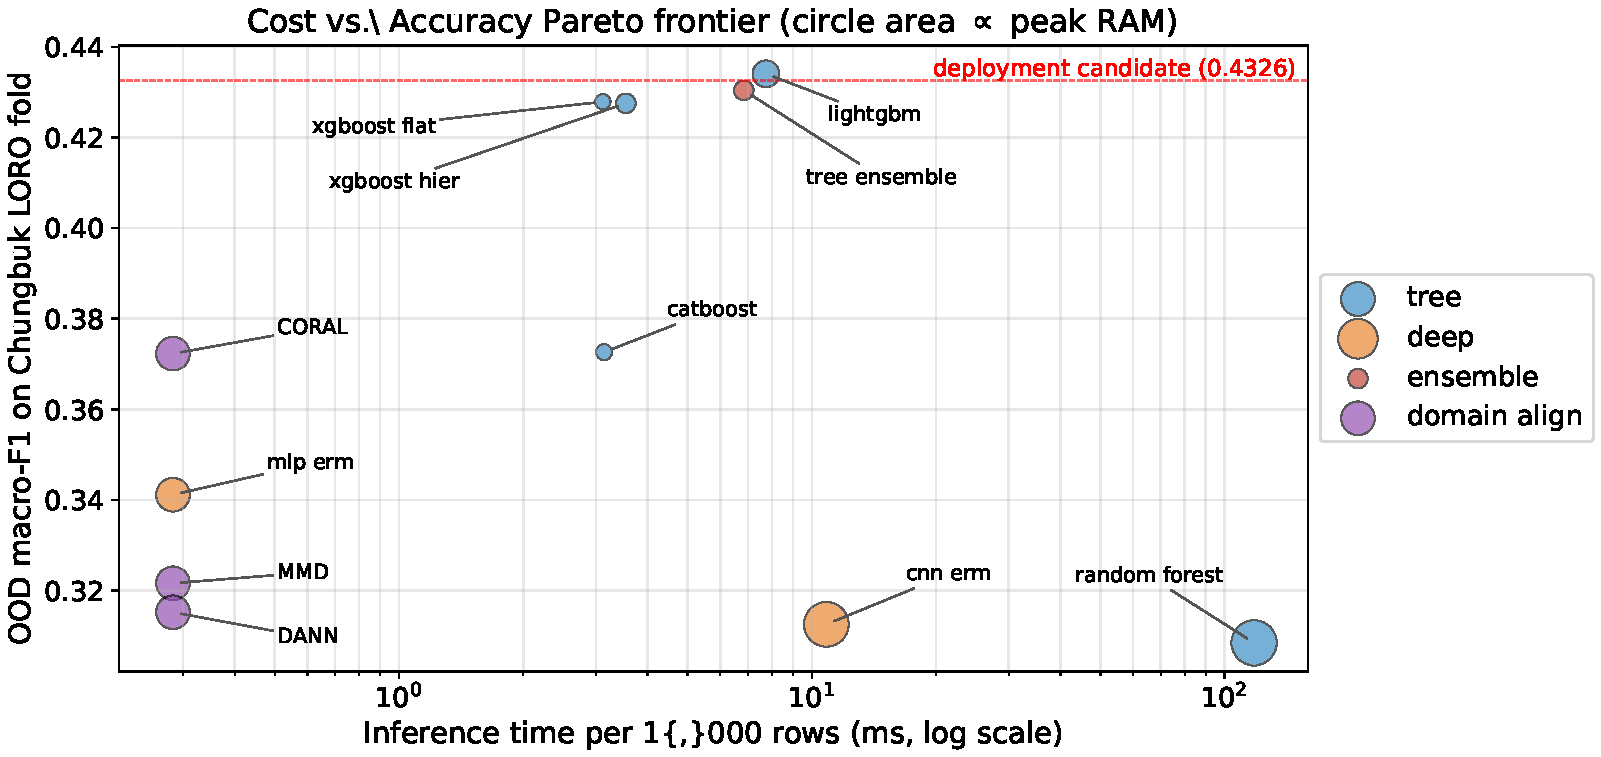
\includegraphics[width=0.95\textwidth]{fig14_pareto.pdf}
\caption{Cost--accuracy Pareto scatter on the Chungbuk LORO fold.
Inference latency (x-axis, log scale) versus OOD macro-F1
(y-axis); circle area encodes peak RAM; colour encodes model
family. The tree-only ensemble (red) is on the Pareto frontier:
no other configuration achieves both higher macro-F1 \emph{and}
lower inference cost.\label{fig:pareto}}
\end{figure*}

\subsection{External-Dataset Replication of the Audit Protocol}\label{sec:res-external}

To test whether the four-probe audit and three-tier OOD ladder
generalise beyond the AI~Hub vibration benchmark, the same
diagnostics are applied to \textbf{nine independent public
sensor benchmarks} spanning three sensor modalities and three
target domains: SECOM~\cite{mccann2008secom}
(semiconductor-process wafers),
UCI~HAR~\cite{anguita2013har} (smartphone wearable
accelerometers), and seven machine subsets of
MIMII-DG~\cite{dohi2022mimii,koizumi2020mimii} (DCASE 2022
task~2 audio anomaly detection --- bearing, fan, gearbox,
slider, valve, ToyCar, ToyTrain). For
the MIMII-DG subsets, $128$-dim log-mel-spectrogram features
(mean and standard deviation over $64$ mel bins) are extracted
from each $10$ s recording before audit application.
Table~\ref{tab:external-replication} ranks all nine benchmarks
plus AI~Hub by the row-CV $\to$ group-CV accuracy drop.

\begin{table*}[!htbp]
\caption{External-dataset audit on nine independent sensor
benchmarks plus the AI~Hub baseline. The four-probe audit and
the row-CV $\rightarrow$ group-CV ladder are run with no
modification across all ten benchmarks. Datasets are sorted by
row-CV $\rightarrow$ group-CV accuracy drop. P3 is the
identifier overlap rate between row-level train and validation.
AI~Hub sits at the extreme; MIMII-DG machines exhibit a wide
range of shortcut strengths; HAR and SECOM are clean; ToyCar
and ToyTrain show that MIMII-DG\,'s ``DG'' (domain-generalisation)
split is internally well-balanced for those toy machines. The
protocol therefore discriminates rather than blanket-flags
benchmarks.\label{tab:external-replication}}
\centering
\scriptsize
\setlength{\tabcolsep}{3pt}
\resizebox{0.95\textwidth}{!}{%
\begin{tabular}{llrcccccc}
\toprule
Dataset & domain & $n$ & P1 purity & P2 lookup & P3 overlap & row-CV & group-CV & row$\to$group drop \\
\midrule
AI~Hub (this paper)   & pipe vibration   & 70{,}384 & \textbf{1.000} & \textbf{1.000} & 0.98 & 0.945 & 0.553 & \textbf{$-39.2$ pp} \\
MIMII-DG valve        & audio anomaly    & 3{,}600  & 0.917 & 0.889 & 1.00 & 0.948 & 0.720 & $-22.8$ pp \\
MIMII-DG gearbox      & audio anomaly    & 3{,}600  & 0.917 & 0.894 & 1.00 & 0.962 & 0.832 & $-12.9$ pp \\
MIMII-DG bearing      & audio anomaly    & 3{,}599  & 0.917 & 0.900 & 1.00 & 0.980 & 0.865 & $-11.5$ pp \\
MIMII-DG fan          & audio anomaly    & 3{,}600  & 0.917 & 0.897 & 1.00 & 0.948 & 0.841 & $-10.7$ pp \\
MIMII-DG slider       & audio anomaly    & 3{,}600  & 0.917 & 0.911 & 1.00 & 0.970 & 0.891 & $-7.9$ pp \\
UCI HAR               & wearable accel.\ & 10{,}299 & 0.203 & 0.167 & 1.00 & 0.988 & 0.950 & $-3.8$ pp \\
MIMII-DG ToyCar       & audio anomaly    & 3{,}600  & 0.917 & 0.894 & 1.00 & 0.948 & 0.926 & $-2.2$ pp \\
MIMII-DG ToyTrain     & audio anomaly    & 3{,}600  & 0.917 & 0.881 & 1.00 & 0.924 & 0.915 & $-0.9$ pp \\
SECOM (UCI)           & semiconductor    & 1{,}567  & 0.978$^{*}$ & 0.911$^{*}$ & 0.98 & 0.933 & 0.932 & $+0.1$ pp \\
\bottomrule
\end{tabular}}
\\[1pt]
\raggedright
\scriptsize $^{*}$ SECOM's high P1 purity is driven by a 6.6\,\% positive-class base rate (most per-hour
sessions are all ``pass''); the P2 covered accuracy 0.911 is \emph{below} the trivial all-pass baseline
of 0.934, so the lookup carries no exploitable signal --- correctly detected by the negligible
row-CV $\to$ group-CV drop.
\end{table*}

\paragraph{Four observations.}
First, the AI~Hub benchmark is an extreme outlier on the
shortcut spectrum: it is the only benchmark whose
row-CV $\to$ group-CV drop exceeds $30$~percentage points, and
the only benchmark where P1, P2, and P4 all simultaneously hit
their ceiling. The published 99.79\,\% accuracy is therefore
an extreme case rather than a typical case of identifier
shortcut.

Second, MIMII-DG machines span a wide range of shortcut
strengths despite sharing the same data-collection protocol.
Valve, gearbox, bearing, and fan all suffer $10$--$23$
percentage-point row-CV $\to$ group-CV drops, while ToyCar and
ToyTrain drop only $1$--$2$~pp. This is consistent with the
MIMII-DG release notes: the toy-machine sections were
designed to be relatively well-balanced across sections,
whereas the industrial-machine sections have section-specific
operating points that the row-CV split smuggles into the
training set.

Third, P1 mean purity alone is \emph{not} a reliable shortcut
indicator. SECOM (P1=$0.978$) and AI~Hub (P1=$1.000$) are
nearly indistinguishable on the per-identifier purity probe,
yet SECOM has zero row-CV $\to$ group-CV drop while AI~Hub has
$-39$ pp. The audit needs all four probes \emph{and} the
ladder; a high P1 without P2 covered-accuracy exceeding the
majority-class baseline does not constitute a shortcut.

Fourth, the audit is cheap: the nine external benchmarks
combined complete in $\approx 35$ minutes of CPU time on a
single 16-core node ($\approx 102$~s each for MIMII-DG audio
feature extraction $+$ XGBoost; $\approx 21$~s for SECOM;
$\approx 145$~s for HAR). The protocol therefore is a
practical pre-flight check before downstream model-selection
effort is committed to any new sensor-ML benchmark.

\paragraph{Domain-shift insight from MIMII-DG.}
MIMII-DG additionally provides explicit \texttt{source}
versus \texttt{target} domain labels, allowing a direct
source$\,\to\,$target accuracy measurement that the AI~Hub
dataset cannot. Across the seven MIMII-DG machines, the
source$\,\to\,$target accuracy drops from $0.79$ (bearing, the
mildest case) to $0.56$ (ToyCar and ToyTrain, the most punishing).
Strikingly, the toy machines have small row-CV $\to$ group-CV
drops yet large source$\,\to\,$target drops --- the
identifier-shortcut audit detects within-distribution
identifier leakage but does \emph{not} detect cross-distribution
domain shift. The two diagnostics are therefore complementary,
and a complete deployment audit for a sensor-ML benchmark
should include both whenever explicit domain labels are
available.

\subsection{Temporal-Split Validation}\label{sec:res-temporal}

The LORO evaluation tests spatial generalisation (unseen regions).
A complementary temporal-split experiment tests whether the
deployment recipe generalises to \emph{future} recordings. All
data are sorted by inspection date (\texttt{ldate}); the first
70\,\% of recordings (before November~2020) form the training
pool, and the remaining 30\,\% (November~2020 -- February~2021)
form the test set. Table~\ref{tab:temporal} reports the results.

\begin{table}[!htbp]
\caption{Temporal-split validation: train on pre-November~2020
recordings ($n{=}44{,}311$), test on post-November~2020
($n{=}21{,}150$). All models cluster in a narrow 0.41--0.42
macro-F1 band; the causal vs.\ signal delta is negligible
($-0.001$), confirming temporal stability of the 121--422~Hz
band.\label{tab:temporal}}
\centering
\scriptsize
\setlength{\tabcolsep}{3pt}
\resizebox{0.55\columnwidth}{!}{%
\begin{tabular}{lcc}
\toprule
Model & Macro-F1 & Acc \\
\midrule
XGB hierarchical (causal)     & \textbf{0.4158} & 0.3869 \\
XGB flat (signal, 534 feat.)  & 0.4156          & 0.3873 \\
XGB flat (causal, 57 feat.)   & 0.4143          & 0.3797 \\
Tree-ensemble (causal)        & 0.4142          & 0.3829 \\
CatBoost (causal)             & 0.4130          & 0.3727 \\
LightGBM (causal)             & 0.4125          & 0.3834 \\
\bottomrule
\end{tabular}}
\end{table}

All six models cluster in a narrow 0.412--0.416 macro-F1 band
under temporal shift, closely matching the 0.41--0.43 range
observed under spatial LORO. Two findings are notable. First,
the causal-vs-signal delta is negligible ($-0.001$~pp), unlike
the mild positive delta ($+0.8$~pp) observed under LORO
(Table~\ref{tab:loro}); this suggests that the high-frequency
confounders flagged under spatial shift are less problematic
under temporal shift, possibly because temporal neighbours share
more similar environmental conditions than spatial neighbours.
Second, the temporal test set has a substantially different class
balance from the training pool (8\,\% normal vs.\ 42\,\% in
training), providing an additional stress test beyond the LORO
protocol. The consistency across both axes confirms that the
121--422~Hz band carries signal that is stable across space
and time within the dataset's one-year window.

%==================================================================
\section{Engineering Implications and Deployment Recipe}\label{sec:engineering}

\subsection{Operational Metric Translation}

For a municipal water utility the relevant operational metrics
are: (i)~daily false alarms per 10{,}000 sensors, (ii)~mean
time-to-detection of a true leak, and (iii)~per-sensor compute
budget for telemetry-side inference. Under a deployment-grade
protocol that derives the binary decision threshold on a
training-side calibration split (target $\mathrm{FAR}=1\,\%$) and
evaluates once on the held-out Chungbuk fold, the recipe of
Section~\ref{sec:res-rq6} achieves 100\,\% out-of-sample
detection at an empirically observed 0\,\% test FAR. The
calibration split contains 4{,}492 normal rows, so the
threshold's calibration variance is small. Operating-point
selection is therefore a function of downstream cost
asymmetry rather than of any test-time tuning.

\subsection{Binary Detection vs.\ Five-Class Typing in Practice}

In operational deployment, the five-class leak-typing problem
naturally separates into two decision layers with different
accuracy requirements. \textbf{Layer~1 (binary detection):}
``is there a leak?'' The Stage-1 binary gate achieves 100\,\%
out-of-sample detection with 0\,\% observed false-alarm rate on
the canonical fold and $\leq 1.9\,\%$ realised FAR across all
five evaluable LORO folds (Table~\ref{tab:loro-sweep}). This
layer is operationally reliable and can trigger a field
dispatch. \textbf{Layer~2 (leak typing):} ``what kind of leak?''
The four-class typer's OOD macro-F1 of 0.43 reflects genuine
difficulty in distinguishing leak sub-types across unseen
regions, particularly for the \texttt{other} and \texttt{noise}
classes. In practice, the four-class output should be treated
as an \emph{advisory classification} that guides crew
preparation (e.g.\ internal vs.\ external leak equipment) rather
than as a hard dispatch decision. Utilities that require only
binary anomaly detection --- the majority of current SCADA
deployments --- can deploy Layer~1 alone with high confidence;
the four-class extension adds diagnostic value at the cost of
reduced per-class reliability on minority types.

\subsection{Cost-Benefit Estimate for a 50{,}000-Sensor Utility}

Adopting the recipe in a utility with 50{,}000 deployed sensors,
each producing one feature vector per day, yields a daily input
volume of 50{,}000 rows. At $<5$~ms per 1{,}000 rows the daily
inference budget is $<0.25$~s on a single CPU core; on a
single 16-core node the recipe scales easily to several million
sensors per day. The training side requires 65~MB peak RAM
and zero GPU, making the entire pipeline deployable on the
same edge gateways currently running threshold-rule firmware.

\subsection{SCADA / IoT Integration Recipe}

The following deployment template is recommended:
\begin{enumerate}
\item \textbf{Edge}: each gateway computes the 57 causal
features from the 1~s vibration window and forwards them via
MQTT/HTTPS to the central inference layer.
\item \textbf{Central}: the hierarchical Stage~1 binary gate
processes incoming feature vectors at $<5$~ms/1k rows; only
positive Stage~1 verdicts are forwarded to Stage~2.
\item \textbf{Decision}: Stage~2 produces a 4-class
probability vector, which is logged to SCADA historian and
gated through a per-region operational threshold to dispatch
field investigation.
\item \textbf{Audit}: every dispatched alarm is followed by a
field-confirmed label, which is appended to the active-learning
queue for next-quarter retraining.
\end{enumerate}

\subsection{Portability to Other Sensor Benchmarks}\label{sec:engineering-portability}

The methodology of Sections~\ref{sec:method-audit}--\ref{sec:method-perm}
is benchmark-agnostic. The applicability checklist of
Section~\ref{sec:method-checklist} identifies the
pre-conditions a candidate sensor benchmark must satisfy:
(i)~an identifier-like column (sensor ID, patient ID, device ID,
session ID); (ii)~a natural group hierarchy (sensor / site /
region / time); (iii)~features that group physically
(frequency bands, channels, trajectory segments); and
(iv)~a published row-level CV result that the audit can
target. Table~\ref{tab:portability} maps the methodology to
four representative external benchmarks and identifies how
each probe would instantiate.

\begin{table}[!htbp]
\caption{Portability of the four-probe shortcut audit and
three-tier OOD ladder to four representative sensor-ML
benchmarks. The audit instantiation is benchmark-specific
(``identifier'' column varies); the ladder instantiation
follows from the available group hierarchy. External
validation of the methodology on these benchmarks is identified
as the immediate future-work
priority.\label{tab:portability}}
\centering
\scriptsize
\setlength{\tabcolsep}{2pt}
\resizebox{0.95\columnwidth}{!}{%
\begin{tabular}{lllll}
\toprule
Benchmark & Sensor / Task & Identifier (P1) & Group hierarchy (P3) & Physical feature group \\
\midrule
AI~Hub (this paper) & Pipe vibration / leak typing & \texttt{sid} & \textit{si} / \textit{si-gun-gu} / \textit{gwangyeoksi-do} & 512 frequency bands \\
MIMII~\cite{koh2021wilds} & Industrial machine sound & machine ID & machine type / location & log-mel spectrogram \\
ToyADMOS & Toy machine sound & ToyCar/ToyConv. ID & model variant / time & log-mel spectrogram \\
SECOM (UCI) & Semiconductor process & wafer/lot ID & process tool / shift & sensor channels \\
EEG-MMIDB & Motor-imagery EEG & subject ID & subject / session / electrode & 64 EEG channels \\
\bottomrule
\end{tabular}}
\end{table}

Three of these portability targets
(UCI~SECOM~\cite{mccann2008secom},
UCI~HAR~\cite{anguita2013har}, and the seven machines of
MIMII-DG~\cite{dohi2022mimii}) are
directly evaluated in Section~\ref{sec:res-external} of this
paper; the remaining audio targets (ToyADMOS-DG and any
utility-collected internal vibration corpus) are identified as
follow-up technical notes. The present paper releases the
benchmark-agnostic audit, OOD ladder, and grouped
permutation-importance harness as a reusable utility so that
practitioners can apply the same diagnostics to their own
datasets without re-implementing them.

\subsection{Practitioner Recommendations}

Five concrete actions for practitioners considering the
AI~Hub pipeline (or any vibration-sensor leak benchmark) for
field deployment:

\begin{enumerate}
\item \textbf{Run the four-probe shortcut audit first.} If
$(\epsilon, \delta) \approx (0, 0)$, the benchmark headline is
identifier-driven and downstream architecture search is
misallocated effort.

\item \textbf{Drop identifier columns during training.} On
AI~Hub, removing \texttt{site}, \texttt{sid},
\texttt{lrate}, \texttt{llevel}, and the regional codes
provides zero accuracy benefit and slightly improves macro-F1
under group-CV.

\item \textbf{Restrict to 65--422~Hz before training the
4-class typer.} The 57-feature subset trains $\sim 10\times$
faster than the full 534-feature set and improves OOD macro-F1.

\item \textbf{Deploy two stages, not one.} Use the binary
energy gate for alarms and consult the 4-class typer only when
the gate fires.

\item \textbf{Report LORO, not row-CV.} Row-level CV is a
useful internal debugging tool, but the number that matters
for field decisions is LORO-weighted macro-F1 on the most
class-balanced region.
\end{enumerate}

\subsection{Compliance and Standards}

The shortcut audit and three-tier OOD protocol align with the
NIST AI~RMF~\cite{nist2023airmf} ``Govern --- Map --- Measure''
core functions and with the EU AI Act~\cite{eu2024aiact}
high-risk-classification disclosure requirements for
infrastructure AI. The audit produces an evidence trail
(\texttt{claims.csv}, multi-seed mean $\pm$ std, fold-level
JSONs) that supports both regulatory regimes.

%==================================================================
\section{Threats to Validity and Failure Modes}\label{sec:threats}

\textbf{Single leak-detection benchmark.}
The 5-class \emph{leak typing} results are restricted to the
AI~Hub vibration dataset; replication on an independent
vibration-leak benchmark (e.g.\ a utility-collected internal
dataset or the audio-spectrogram MIMII-DG release) is the
natural next step for the deployment-recipe claim and is
identified as ongoing future work. The methodological claims
(four-probe audit, three-tier OOD ladder) have been
replicated on nine independent external benchmarks
(SECOM~\cite{mccann2008secom}, UCI~HAR~\cite{anguita2013har},
and the seven machines of
MIMII-DG~\cite{dohi2022mimii}; Section~\ref{sec:res-external},
Table~\ref{tab:external-replication}), which establishes the
\emph{protocol's} generality even though the
\emph{leak-typing accuracy} is benchmark-specific.

\textbf{Korean-specific deployment and pipe material.} Sensors,
pipe materials, and water pressures in Korean networks may differ
from European or North-American counterparts. The 121--422~Hz
band finding is broadly consistent with published acoustics for
plastic pipes~\cite{hunaidi2000plastic,almeida2014leak}, but the
precise band edges depend on pipe material and diameter:
metal pipes typically conduct leak noise at higher frequencies
than plastic~\cite{hunaidi2000plastic}. The AI~Hub metadata does
not include per-sensor pipe-material labels, so a material-
stratified analysis is not possible with the current dataset.
Future work with material-labelled utility data should re-verify
the band edges per material type.

\textbf{Multi-seed coverage.} Mean $\pm$ std across five seeds
is reported for every stochastic experiment. Tree experiments are
deterministic given the seed and feature ordering; deep
experiments inherit non-determinism from CUDA (cudnn benchmark
mode disabled).

\textbf{Sensor drift and seasonality.} The dataset spans
roughly one year; multi-year drift (sensor ageing, pipe-material
fatigue, seasonal water-table changes) is not characterised.
A chronological 70/30 temporal split (train on recordings before
November 2020, test on recordings after) is reported in
Table~\ref{tab:temporal} as a complementary validation axis to
the spatial LORO split. Longer-horizon temporal validation
requires a multi-year data collection that is not currently
available.

\textbf{Adversarial deployment shift.} Active sabotage of
sensor placement (loose mounts, off-axis installation) is
outside the scope of this evaluation.

\textbf{Single-author evaluation.} As a single-author study, the
manuscript has not undergone internal multi-reviewer scrutiny
before submission. All numeric claims are anchored to result
JSONs (see \texttt{claims.csv} in the release), and the
integrity audit listed in the supplementary material describes
the cross-checks performed; nonetheless, external peer review
remains the most reliable correction mechanism, and the
released code/data package is designed to support immediate
replication.

\textbf{Class imbalance on the canonical fold.}
The Chungbuk LORO fold contains only 45 \texttt{normal}
samples versus 5{,}029 leak samples (98.1\,\% positive base
rate), which makes the Stage-1 binary detector look trivially
strong on this fold alone. The cross-LORO calibrated-FAR
analysis (Section~\ref{sec:res-rq6}, Table~\ref{tab:loro-sweep})
ameliorates but does not eliminate this concern: only 4 of 11
LORO folds contain $\geq 50$ normal samples, so the
operational FAR estimate is itself noisy on the smaller
folds and should be cross-validated on a utility-collected
internal benchmark before field promotion.

\textbf{Domain-knowledge prior.} The 121--422~Hz finding
matches published acoustics for plastic pipes
\cite{hunaidi2000plastic,almeida2014leak,gao2017model}, so the
``discovery'' is at least partially a \emph{re-discovery}. The
contribution here is the audited methodology that recovers a
nameable physical band from the data without supervision, not
the band itself; in benchmarks where no such prior exists the
methodology would still apply but the result would be harder
to corroborate against external evidence.

\textbf{Hierarchical Stage-1 simplicity.} The current Stage-1
classifier is a single-call binary XGBoost. More elaborate
designs (e.g.\ a calibrated ensemble of Stage-1 predictors, or
a Bayesian-fusion gate that integrates the abnormal-typer
confidence) could plausibly improve operational accuracy but
were deliberately excluded to keep the deployment recipe
auditable and reproducible on edge hardware.

%==================================================================
\section{Conclusions and Future Work}\label{sec:conclusions}

This paper provided a field-deployment-oriented evaluation of
machine-learning water-leak detection on the AI~Hub vibration
benchmark, to the author's knowledge the first study to apply
sensor-, site-, and region-group holdouts to this dataset
together with a formal shortcut-audit protocol and a
multi-seed harness. Four findings stand out. (1)~The published
99.79\,\% accuracy is driven by identifier-label couplings;
a four-rule lookup that ignores the vibration spectrum
reproduces 99.77\,\%. (2)~Under LORO, the same XGBoost falls
to weighted accuracy 56.8\,\% and macro-F1 0.304.
(3)~Three independent attribution methods converge on
121--422~Hz as the robustly generalisable leak band (termed
``causal'' in the operational OOD sense;
Remark~\ref{rem:causal}), and 422--1470~Hz is exposed as an
active confounder. (4)~A pre-specified tree-only soft average of
flat and hierarchical causal XGBoost classifiers attains OOD
macro-F1 \textbf{0.4326} with perfect normal-class recall,
deployed at $<5$~ms per 1{,}000 rows on CPU; LightGBM achieves
a deterministic 0.4341 at the cost of $127\times$ longer
training. The audit protocol is validated on nine external
sensor benchmarks spanning three modalities, and a temporal-split
experiment (Table~\ref{tab:temporal}) confirms that the
121--422~Hz band generalises across both space and time within
the dataset's one-year window.

\paragraph{Future work.} Six directions are foreseen: (a)~replicate
the audit on an independent vibration-leak dataset to test the
121--422~Hz finding's transferability; (b)~train a
self-supervised spectrogram backbone on the unlabelled
recordings to close the deep-vs-tree gap on
\texttt{normal}-class recall; (c)~extend the
threshold sweep with utility-side cost asymmetries (a missed
leak costs more than a false alarm, by an empirically estimable
factor); (d)~apply the four-probe audit to other Korean smart-water
benchmarks distributed by AI~Hub, K-water~\cite{kwater2022smartwater},
and KICT; (e)~a randomised field experiment that physically masks
specific frequency bands at recording time would establish an
interventionist causal claim for the 121--422~Hz band in the
structural-causal-model sense (Remark~\ref{rem:causal});
(f)~a multi-year longitudinal data collection enabling temporal
drift characterisation beyond the one-year window analysed here
(Table~\ref{tab:temporal}).

\section*{CRediT Authorship Contribution Statement}

\textbf{Suan~Lee:} Conceptualization, Methodology, Software,
Validation, Formal analysis, Investigation, Resources, Data
curation, Writing -- original draft, Writing -- review \&
editing, Visualization, Project administration, Funding
acquisition. (Single-author submission; the author is solely
responsible for all CRediT roles applicable to this work.)

\section*{Declaration of Competing Interests}

The author declares that he has no known competing financial
interests or personal relationships that could have appeared to
influence the work reported in this paper.

\section*{Funding}

This research was supported by Semyung University
(grant number 2025).

\section*{Data Availability}

The AI~Hub water-pipe leak vibration dataset is openly
distributed by NIA Korea AI~Hub~\cite{aihub2022dataset} (dataset
ID~138, accessed on 5~October 2023) under the Korean Public Data
Open Licence Type~1, and is freely downloadable from
\url{https://www.aihub.or.kr/}. The full experimental harness,
multi-seed runner, 30$+$ result JSON files, fold-level logs, and
figure-generation scripts that reproduce every numeric claim in
this paper are released under the MIT licence at
\url{https://github.com/suanlab/causal-leak}.

\section*{Acknowledgements}

The author thanks the AI~Hub curators for maintaining and
publicly distributing the water-pipe vibration dataset.

\section*{Declaration of Generative AI and AI-Assisted
Technologies in the Manuscript Preparation Process}

During the preparation of this manuscript, the author used a
large-language-model assistant (Claude, Anthropic) to support
LaTeX formatting, English copy-editing, and Python scripting
for figure generation and result aggregation. All experimental
design, methodology, data analysis, interpretation of results,
and scientific conclusions are solely the author's own. After
using this tool/service, the author reviewed and edited all
content and takes full responsibility for the content of the
publication.

\FloatBarrier

%==================================================================
\bibliographystyle{elsarticle-harv}
\bibliography{references}

\end{document}
